\documentclass[11pt, a4paper, twoside, openright]{book}
% Load packages 
\usepackage{amsmath, amssymb,mathrsfs}
\usepackage[T1]{fontenc}
\usepackage[utf8]{inputenc}
\usepackage{blindtext}
\usepackage{graphicx}
\usepackage[dvipsnames]{xcolor}
\usepackage{listings} % format code
\usepackage{multicol}
\usepackage{makecell} % Allow text to wrap in tables
\usepackage{booktabs} % Rulers in tables
\usepackage{changepage}
\usepackage{indentfirst}
\usepackage{float}
\usepackage{setspace}

% Manage bibliography
\usepackage[
backend=biber,
style = numeric-comp,
maxnames = 2,
doi=false,
isbn=false,
url = false,
eprint = false,
sorting=none
]{biblatex}
\addbibresource{Literature overview.bib}
\addbibresource{other-papers.bib}
\addbibresource{Rational polynomial models.bib}
\addbibresource{background_literature.bib}

% Set page layout
\usepackage{geometry} %[showframe]
\geometry{
a4paper,
%includeheadfoot,
%total={190mm,257mm},
headheight = 10mm,
footskip = 15mm,
inner = 25mm,
outer = 60mm,
top=25mm,
bottom=20mm,
marginparwidth = 50mm
}
\savegeometry{main_body}

\geometry{
a4paper,
headheight = 10mm,
footskip = 15mm,
inner = 25mm,
outer = 25mm,
top=25mm,
bottom=20mm,
marginparwidth = 0mm
}
\savegeometry{full_page}

\geometry{
a4paper,
headheight = 10mm,
footskip = 15mm,
inner = 25mm,
outer = 10mm,
top=25mm,
bottom=20mm,
marginparwidth = 0mm
}
\savegeometry{no_margin}
\loadgeometry{main_body}

% Set the captions
\usepackage[font={it, small}]{caption}
% Abilitate continuation to new line
% \captionsetup[figure]{labelfont=bf}
% \DeclareCaptionLabelFormat{continued}{#1~#2\ (continued)}
% \captionsetup[ContinuedFloat]{labelformat=continued}


% Set up code blocks env
\usepackage{listings}
\usepackage{xcolor}
\definecolor{codegreen}{rgb}{0,0.6,0}
\definecolor{codegray}{rgb}{0.5,0.5,0.5}
\definecolor{codepurple}{rgb}{0.58,0,0.82}
\definecolor{backcolour}{rgb}{0.95,0.95,0.92}
\lstdefinestyle{mystyle}{
    backgroundcolor=\color{backcolour},   
    commentstyle=\color{codegreen},
    keywordstyle=\color{magenta},
    numberstyle=\tiny\color{codegray},
    stringstyle=\color{codepurple},
    basicstyle=\ttfamily\footnotesize,
    breakatwhitespace=false,         
    breaklines=true,                 
    captionpos=b,                    
    keepspaces=true,                 
    numbers=left,                    
    numbersep=5pt,                  
    showspaces=false,                
    showstringspaces=false,
    showtabs=false,                  
    tabsize=2
}
\lstset{style=mystyle}

% Choose main font for the text
% \usepackage{XCharter}
\usepackage{mlmodern}
%\usepackage{fourier}
% \usepackage{helvet}
%\usepackage{bookman}
%\usepackage{lexend}

% \usepackage{oswald}
% \usepackage{kpfonts}


% Create custom command for settimang fonts
% \newcommand{\helvetfont}{\fontfamily{phv}\selectfont}

% \newcommand{\bookfont}{\fontfamily{pbk }\selectfont}

% \newcommand{\palafont}{\fontfamily{ppl }\selectfont}

% Custommize headers and footers
\usepackage{fancyhdr}
\pagestyle{fancy}
\addtolength{\headwidth}{\marginparwidth}%{.1cm}
\addtolength{\headwidth}{.1cm}
\renewcommand{\chaptermark}[1]{\markboth{Chapter \thechapter.\ #1}{}}
\renewcommand{\sectionmark}[1]{\markright{\thesection.\ #1}}
\fancyhf{}
\fancyhead[RO]{\rightmark}
\fancyhead[LE]{\leftmark}
\fancyfoot[C]{\thepage}
\renewcommand{\headrulewidth}{0pt}

%\usepackage{fancyhdr}
% \pagestyle{fancy}
% \fancyhead{} % clear all header fields
% %\renewcommand{\chaptermark}[1]{\markboth{#1}{}}
% %\renewcommand{\sectionmark}[1]{\markboth{#1}{}}
% \fancyhead[LEH]{\thepage \qquad \leftmark}
% \fancyhead[ROH]{\rightmark \qquad \thepage }
% \fancyfoot{}
% \renewcommand{\headrulewidth}{0pt}

% Remove numbers from empty pages
\let\origdoublepage\cleardoublepage
\newcommand{\clearemptydoublepage}{\clearpage{\pagestyle{empty}\origdoublepage}}
\let\cleardoublepage\clearemptydoublepage


% Format the titles style
\setcounter{secnumdepth}{2}

% \usepackage{titlesec}

% \newcommand{\oswald}{\fontfamily{oswald}\selectfont}
% % SECTION
% \titleformat{\section}
%   {\oswald\selectfont\Large}
%   {\thesection}{1em}{}

% % SUBSECTION
% \titleformat{\subsection}
%   {\fontfamily{cmr}\selectfont\large}
%   {\thesubsection}{1em}{}

% \newlength\fullchapwidth
% \setlength\fullchapwidth{%
%   \dimexpr\textwidth+\marginparsep+\marginparwidth\relax
% }

% \titleformat{\chapter}[display]
%   {\Huge\bfseries}
%   {\fontfamily{pbk}\selectfont\scalebox{3}{\color{lightgray}\ \thechapter}
%   }
%   {0pt}
%   {}

% \makeatletter
% \titleformat{\part}[display]
%   {\Huge\scshape\filright}
%   {\partname~\thepart:}
%   {20pt}
%   {\thispagestyle{epigraph}}
% \makeatother
% \setlength\epigraphwidth{.6\textwidth}

% \titleformat{\section}[display]
%   {\fontfamily{phv}\selectfont\scalebox{1}{\color{lightgray}\thesection}\quad}
%   {0pt}
%   {}

% \titleformat{\subsection}[block]
%   {\Large\bfseries\palafont}
%   {\fontfamily{pbk}\selectfont\scalebox{0.8}{\color{lightgray}\thesubsection}\quad}
%   {0pt}
%   {}

% \titleformat{\subsubsection}[block]
%   {\normalsize\bfseries\palafont}
%   {\fontfamily{qag}\selectfont\scalebox{0.8}}
%   {0pt}
%   {}

% Format tables of content

% Main ToC
%\usepackage{titletoc}
 

% Mini ToC for each chapter
% \usepackage[nohints,tight]{minitoc} 
% \setcounter{minitocdepth}{1}
% \renewcommand{\mtifont}{\large\bookfont}
% \renewcommand{\mtcfont}{\small\bookfont}
% \renewcommand{\mtcSfont}{\small\bookfont}
% \renewcommand{\mtcSSfont}{\small\bookfont}
% \renewcommand{\mtcSSSfont}{\small\bookfont}


% % Create custom environment for whill width content
% \usepackage{changepage}
% % The following code should be used *after* any changes to the margins and
% % page layout are made (e.g., after the geometry package has been loaded).
% \newlength{\fullwidthlen}
% \setlength{\fullwidthlen}{\marginparwidth}
% \addtolength{\fullwidthlen}{\marginparsep}

% \usepackage{fullwidth}

% \captionsetup{
%   justification=raggedright,
%   labelfont={color=Gray,bf},
%   font=small}

% \newenvironment{fullwidthfigure}[1][]{
%   \begin{figure}[#1]
%   \noindent
%   \checkoddpage
%   \ifoddpage
%     \hspace*{-\oddsidemargin}\hspace*{-1in}%
%   \else
%     \hspace*{-\evensidemargin}\hspace*{-1in}%
%   \fi
%   \bgroup
% }{
%   \egroup
%   \end{figure}
% }


% -------------------------------------------------------
% MARGIN CAPTIONS (kaobook / tufte style)
% -------------------------------------------------------

% % caption appearance
% \captionsetup{
%   font=small,
%   labelfont=bf,
%   justification=raggedright,
%   singlelinecheck=false
% }

% % floatrow configuration: captions in margin
% \floatsetup[figure]{
%   margins=raggedright,
%   capposition=beside,
%   capbesideposition={right,top},
%   capbesidewidth=\marginparwidth
% }
% \usepackage{ifoddpage}

% \newcommand{\setmarginfigurecaption}{%
%   \checkoddpage
%   \ifoddpage
%     \floatsetup[figure]{capbesideposition={right,top}}
%   \else
%     \floatsetup[figure]{capbesideposition={left,top}}
%   \fi
% }


% -------------------------------------------------------
% WIDE FIGURE — twoside aware (pdflatex safe)
% expands into OUTER margin only
% -------------------------------------------------------

\usepackage{ifoddpage}
\usepackage{changepage}

% compute margin extension
\newlength{\outermarginwidth}
\setlength{\outermarginwidth}{\marginparwidth}
\addtolength{\outermarginwidth}{\marginparsep}

\newenvironment{widefigure}[1][htbp]
  {\begin{figure}[#1]
   \checkoddpage
   \ifoddpage
     % recto page → expand right
     \begin{adjustwidth}{0pt}{-\outermarginwidth}
   \else
     % verso page → expand left
     \begin{adjustwidth}{-\outermarginwidth}{0pt}
   \fi
   \centering
  }
  {\end{adjustwidth}
   \end{figure}
  }

% \usepackage{etoolbox}

% \AtBeginEnvironment{figure}{\setmarginfigurecaption}

% Set sidenotes
\usepackage{marginnote}

% ensure outer-margin placement in twoside
\reversemarginpar

\newcounter{sidenote}

\newcommand{\sidenote}[1]{%
  \refstepcounter{sidenote}%
  \textsuperscript{\thesidenote}%
  \marginnote{\footnotesize\textsuperscript{\thesidenote}\,#1}%
}



% \usepackage{adjmulticol}
% \newenvironment{TwoCol}{\small\begin{adjmulticols}{2}{0in}{-2in}}{\end{adjmulticols}}
% \newenvironment{OneCol}{\small\begin{adjmulticols}{1}{0in}{-2in}}{\end{adjmulticols}}

% Set rules for links
\usepackage[hidelinks]{hyperref}
\hypersetup{
    colorlinks,
    linkcolor={black},
    citecolor={blue!50!black},
    urlcolor={blue!80!black}
}

\title{PhD thesis \\ 
Dynamic Electrochemical Impedance Spectroscopy for Energy Storage Applications: \\ from Electrode Kinetics to Cell Degradation}
\author{Federico Scarpioni}

\begin{document}

\input{customization_mainmatter}

%\begin{titlepage}
\thispagestyle{empty}
% \centering

% -------------------------------------------------
% TITLE
% -------------------------------------------------
\vspace*{1cm}
\begin{spacing}{2.2}
{\noindent\huge
Dynamic Electrochemical Impedance Spectroscopy for Energy Storage Applications:  from Electrode Kinetics to Cell Degradation
}\par
\end{spacing}

\vspace{4cm}

% -------------------------------------------------
% Faculty / University block
% -------------------------------------------------

{\noindent\large
Vom Fachbereich Produktionstechnik\\[0.5em]
der\\[0.5em]
\textbf{Universität Bremen}
\par}

\vspace{1.5cm}

% -------------------------------------------------
% Degree block
% -------------------------------------------------

{\noindent\large
zur Erlangung des Grades\\[0.5em]
\textbf{Doktor der Ingenieurwissenschaften (Dr.-Ing.)}\par}

\vspace{1.5cm}

% -------------------------------------------------
% Author
% -------------------------------------------------

{\noindent\large
Dissertazion\\[0.5em]
Von\\[0.5em]
\textbf{Federico Scarpioni}
\par}

\vspace{\fill}

% -------------------------------------------------
% Reviewers
% -------------------------------------------------

{\noindent\normalsize
Gutachter*innen:\\[0.5em]
Prof. Fabio La Mantia\\[0.5em]
Prof. Dr.-Ing. Julia Kowal, Technische Universität Berlin
\par}

% \vspace{1.5cm}

% -------------------------------------------------
% Defense date
% -------------------------------------------------

% {\noindent\normalsize
% Tag der mündlichen Prüfung:\\[0.5em]
% TT.MM.JJJJ
% \par}

% \vfill

\end{titlepage}
\maketitle

\frontmatter

\dominitoc 
\tableofcontents

\mainmatter

\chapter{Introduction}

% Hook: Electric vehicles need fast charging, long life and safety opration. Understanding battery degradation and side reactoins require monitoring intenral processes during operation.


% Batteries and why impedance matters

The transition to electric mobility and renewable energy storage demands batteries with high energy density, fast charging capability, long operational lifetime and stringent safety requirements. Lithium-ion batteries have dominated the market for portable electronics and are now the technology of choice for electric vehicles, electrical grid stabilization and renewable energy storage. Yet, significant challenges remain in understanding and predicting their degradation mechanisms during operation. Battery aging is a complex interplay of processes occurring at multiple time scales from fast charge transfer reactions at electrode-electrolyte interfaces (microseconds to milliseconds) to slow solid-state diffusion and mechanical degradation (seconds to hours). The understanding and predeiction of a battery, a dynamical system, can be performed from experiment in the time or frequency domain; the latter allowing a much effective way of separating processes at multiple time scale with one simple experiment.

In electrochemistry, the frequency domain identification technique is referred as Electrochemical Impedance Spectroscopy (EIS), excensivly used in battery reserach. By measuring the frequency-dependent response of a battery to small alternating current or voltage perturbations, EIS separates overlapping processes based on their characteristic time constants. A single impedance spectrum encodes information about charge transfer resistance, double-layer capacitance, solid-state diffusion, and interfacial phenomena across a frequency range typically spanning from millihertz to kilohertz. This multi-scale view makes EIS invaluable for battery diagnosis, state-of-health estimation, and mechanistic studies.

% Current state and limitations
However, conventional EIS measurements require the battery to be in a stationary state where the system state (the set of its properties) do not change during the measurement time. For a full spectrum covering six or seven decades of frequency, this requirement translates to measurement times of 30 minutes to several hours. During battery cycling, interrupting the charge or discharge to perform EIS introduces significant overhead time and alters the electrochemical and thermal state of the cell. As a result, operando impedance measurements have been limited to either: narrow frequency bands in the middle to high range (above 1 Hz), which sacrifices the information of transport, or sparse equilibrium measurements at fixed states of charge, which miss the continuous evolution of degradation during long-term cycling. This gap becomes critical when studying phenomena that evolve continuously during cycling: solid-electrolyte interphase growth, lithium plating, particle cracking, or state-dependent kinetics.

% Proposed solution
This thesis addresses this gap by developing a complete methodology for broadband electrochemical impedance spectroscopy in non-stationary conditions. By combining commercial instrumentation with custom automation software and online signal processing, I enable continuous impedance acquisition across seven decades of frequency (10 mHz to 100 kHz) throughout multi-week battery cycling experiments. The methodology removes the stationary-state requirement through multi-frequency perturbation techniques and time-resolved impedance estimation, while solving the practical challenges of data volume (reducing storage requirements by four orders of magnitude through online processing) and multi-channel operation. The open-source software stack makes this capability accessible to other research groups using standard laboratory equipment.

% Explain mulitdisciplinary nature
The development of this methodology required integrating knowledge from multiple disciplines. From electrochemistry, understanding the physical processes at electrode-electrolyte interfaces, charge transfer kinetics, and mass transport phenomena was essential to design appropriate perturbation signals and interpret the resulting impedance spectra. Battery technology knowledge informed the choice of cell geometries, reference electrode designs, and cycling protocols relevant to practical applications. The hardware implementation demanded familiarity with potentiostat operation, waveform generator programming, and high-speed data acquisition systems. Signal processing theory guided the design of multi-sine excitations with optimized crest factors, the implementation of Fourier transform-based impedance estimation, and strategies for managing spectral leakage and noise. System identification concepts—particularly the distinction between stationary and non-stationary systems, transfer function representations, and frequency-domain characterization—provided the theoretical framework for extracting meaningful dynamic models from measured data. Finally, the automation and online processing required advanced programming in Python, including multi-threaded operation, efficient numerical computation with NumPy, and custom hardware interfaces. The parametric analysis of time-varying impedance spectra further demanded expertise in mathematical optimization, including regularized complex nonlinear fitting and model selection criteria. This thesis therefore sits at the intersection of experimental electrochemistry, electrical engineering, digital signal processing, and computational methods—reflecting the inherently multidisciplinary nature of modern battery research.

% Scope statement
The primary focus of this work is the development and validation of the measurement methodology itself. The thesis demonstrates the technique's applicability across multiple electrochemical energy storage systems—commercial batteries, laboratory cells with reference electrodes, Faradaic (intercalation) and non-Faradaic (adsorption) processes—but does not attempt comprehensive mechanistic modeling or full correlation of impedance features to specific degradation modes. Such applications require the foundation that this work provides: a robust, accessible platform for generating the large datasets needed for data-driven battery analysis.


% Thesis outline
This thesis is organized as follows. Part I provides the theoretical framework: Chapter 2 reviews fundamental electrochemistry concepts, Chapter 3 discusses battery technology and characterization methods, Chapter 4 introduces system identification theory for frequency-domain analysis, and Chapter 5 surveys the historical development and state-of-the-art in non-stationary impedance spectroscopy.

Part II describes the methodologies developed in this work: Chapter 7 details the automated data acquisition system, multi-sine signal design, and online impedance calculation, while Chapter 8 presents the analysis approaches for parametric modeling and model selection.

Part III presents results and discussion: Chapter 9 validates the methodology on commercial coin cells throughout their cycling lifetime, Chapters 10-11 demonstrate applications to single-electrode studies (lithium titanium phosphate and electrical double-layer capacitors), and Chapters 12-13 present exploratory measurements on lithium and sodium anodes that reveal methodological challenges for future development. Chapter 14 concludes with a summary of achievements and outlook for future work.

\part{Theoretical framework}
\input{chapters/2_electrochemsitry}
\input{chapters/3_batteries}
\input{chapters/4_identification_dynamic}
\input{chapters/5_dynamic_impedance}
\chapter{Scope of this work}


To make it open source multisine preparation, acquisition, visualization and analysis.

Collect both the high and low part (boardband).

Guess the degrees of freedom from the estimation of the trasnfer function (rational polinomial) using regolarized complex non linear fit of the spectra.



\part{Methodologies}
\chapter{Acquisition of non-stationary impedance}
% \minitoc
\label{ch:acquisition}

This work gives a complete chain for the measurementes of dynamic ipedance spectroscopy:
\begin{itemize}
    \item design and generation of the excitation signal
    \item acquisition of multi-frequency signals with automated set-up
    \item estimation of istantanous impedance from multi-frequency voltage and current signals
    \item analysis of the impedance data for characterization of cells and surface processes
\end{itemize}
This chapter deals with the firs two points \dots

% Introduction and motivation

% Limitation of classical EIS
Electrochemical impedance measurement is traditionally performed under the assumption of stationarity. Its validity vanishes whenever the internal state of the system evolves on comparable or shorter timescales; as occurs during battery charge and discharge, SEI formation, lithiation-induced expansion, or any experiment where the current is not zero for long enough to reach equilibrium.

% Need for broadband, time-resolved measurements
While impedance has been measured in electrochemical storage devices, it was either limited to frequency higher of 1Hz or multisine spanning only 3-4 decades. A full broadband spectra for batteires requires to experiment to be interrupted and waiting for the stationarity condition, which adds overheading time to the battery test making impedance impractical to use in operando conditions.

% Overview of the methodology
This chapter describes the practical methodology and instrumental chain developed to acquire \emph{non-stationary} impedance, i.e. the time-resolved evolution of impedance over several decades of frequency while the system is drifting due to the imposed load. The goal is to obtain continuous impedance spectra over seven orders of magnitude in frequency without interrupting the charge/discharge process.

The principle of the set-up follows the classical design from the literature. A multisine of small amplitude is superimposed to a high-amplitude drift and applied to the cell though a potentiostat. The voltage and current analog signals are sampled at high frequency by a dedicated acquisition device and streamed to a computer. Impedance is estimated from the fouerire trasnform of voltage and current at the frequencies components $\omega_i$ of the multisine excitation. 

The novelty of this work is a methodology that combines the ST-FFT and DMFA to compute the istantanous time-resolved impedance. The first method is used online for the high frequency band and it is followed by a strong downsample, while the secon is applied off-line. The result of the two methods is concatenated to obtain to complete bradband time-resolved spectra.

The methodology combines:
\begin{itemize}
    \item frequency-optimized multisine excitation,
    \item synchronized high-frequency digitization,
    \item real-time spectral estimation and segmentation,
    \item hardware-aware design (memory limits, ADC resolution, synchrony, jitter),
    \item and a Python-based automation framework (called DEIStools) for coordinating potentiostat, waveform generator and oscilloscope.
\end{itemize}

The chapter is organized as follows: 
\begin{itemize}
    \item [\textbf{Section~\ref{sec:hardware}}] describes the experimental hardware chain;
    \item [\textbf{Section~\ref{sec:multisine}}] details the generation, splitting and  optimization of multisine waveforms; 
    \item [\textbf{Section~\ref{sec:sampling}}] addresses sampling, synchronization and spectral leakage;  
    \item [\textbf{Section~\ref{sec:automation}}] summarizes the automation architecture;  
    \item [\textbf{Section~\ref{sec:designrules}}] provides practical guidelines and limitations.
\end{itemize} 

The method for estimating the impedance from multi-frequency data will be the topic of next chapter.

\section{Hardware}
\label{sec:hardware}

% Potentiostat (also intenral architecture?)
% AWG
% Oscilloscope / ADC
% Cabling and isolation
The instrumental set-up used in our labs follows the same design introduced  in section \ref{sec:fft-eis} with a potentiostat interfaced with a dedicated waveform generator, for the excitation, and a dedicate acquisition device for high-frequency sampling and streaming to a computer. 
The multisine excatation is generated as analog voltage signal and injected into the potentiostat where it is superimposed on the main drift. 
It is converted to current though the measurement resistor when the tehnique applied by the potentiostat is galvanostatic.

For this work we assembled multiple set-ups using BioLogic potentiostats, Keysight waveform generators and PicoTech Picoscope acquisition devices. 
The components are connected together using the auxiliary input-output port of the potentiostat: the waveform generator to the input and the scope recieves the voltage and current signals for the synchronous sampling. 
The series and the model might vary experiment by experiment, therefore I will report the exact devices in the next part of the thesis where the results of discussion of multiple application of DEIS are reported. 
The brand, though, remain the same as well as the operating principles and they can be all used with the software solution developed here. 
BioLogic potentiostats have for each channel an auxiliary 9-pin port for the input and output of analog signals. 
For the purpose of this project I was interested in only three: Input (Auciliary In2), voltage monitor and current monitor. The company supplies adapters for the 9-pin to BNC connectors but for me was more practical to build them myself with my requirments. 
A reference for the contruction is available in the Appendix \ref{ap:aux cable}.

\section{Multi-sine design}
\label{sec:multisine}
A multisine is the superposition of many sinusoidal components:
\[
u(t) = \sum_{k=1}^{K} A_k \sin(j2\pi f_k t + \phi_k).
\]
It allows the simultaneous excitation of a large set of frequencies with a 
single time-domain waveform, dramatically reducing the experiment duration.

Obtaining high-quality non-stationary impedance, however, requires careful design of the multisine: frequency grid, crest-factor minimization, amplitude choice and memory constraints of the AWG.

\subsection{Frequencies selection}

The frequencies f must be chosen in a way that one period of the whole multi-sine contains integer numbers of oscillation to ovoid spectral leakage. 
The period is then defined by one oscillation of the sinus with lowest frequency $T=\frac{1}{f_{min}}$.
Every other frequency i-th must satisfy the condition $f_i=k\times f_{min}$, where k is an integer. 
In this work we generate the desired frequencies from an harmonic series of integer to insure the above condition and the possibility to re-use the sequence for multi-sine with different $f_{min}$. 
With the term harmonic sequence I refer to $h_i =\frac{f_i}{f_{min}}$; such that it always starts from 1. The sequence is generated as a logarithmic distribution with a number of point per decade between six and ten; I generally obtain good densities with 8 ponints per decade. 
Lower values gives spares spectra while high values give a denser one. 
Denser spectra are more beneficial for the data regression having more points to cast in the cost function, but the power of the signal increases. 
Eight points seems to me the sweet spots, according to my experience.

\subsection{Amplitude optimization}
\label{sec:amplitude optim}
When the amplitudes are all the same, it is said to have a "flat" multi-sine. 
To question is: how to decide the amplitudes?  It can be achieved via analytical formulas or experimental extrapolation. 
The first case was used in Battistel and Hellemans, with opposite results, making the amplitudes drop logarithmically with the increase of the frequency.  
In my work, I measured the non-stationary impedance for many different chemistry and geometries obtaining quite different results in sense of the module of the impedance. 
Hence, I prefer the approach of choosing the amplitudes based on previous experiment. 
One can just measure a classic stepped-sine impedance with any electrochemical workstation and use its module to calculate the desired input amplitude. 
Alternatively, and more effective for energy storage systems, is to measure the non-stationary impedance firs using a flat multi-sine and then extract from the, often noisy, data the average value and use again its module.
% Moved from the other chapter
Firstly I measured a complete cycle of the battery with dynamic impedance spectroscopy using a equal amplitudes on a test cell (not part of the dataset), and then I used the avarage of the module of such impednace and used it to calculate the amplitudes for the input in order to obtain an output with equal magnitude for each frequencies. 
In mathematical therms, being $|Z_{test}(\omega)|_{avg}$ the avarege of the impedance module, the desired output voltage is unitary for all frequencies, enche the current amplitude follows Ohm's law as:

$$
i(\omega_k) = \frac{1}{|Z_{test}(\omega_k)|_{avg}}.
$$

The output of the waveform generator is a voltage and it is converted to current by the electrochemical workstation during the chronoamperometry technique using the active measurement resistor ($R_m$). 
For this experiments I choose always the same current range of 10 mA for the sequence that translates to a measurement resistor of 100 Ohms. 
Hence for the galvanostatic step the actual peak-to-peak voltage of the generated waveform is 

$$
V(\omega_k) = R_m \times i(\omega_k).
$$

For the potentiostatic step instead the amplitude of the multisine is 

$$
V(\omega_k) = |Z_{test}(\omega_k)|_{avg}.
$$

\subsection{Phase optimization}
The process of identification should be carried out with small amplitude excitation around the operating point point. 
Multi-sine waveforms can often time have large peak to peak total amplitude after optimizing the relative amplitudes derives by the superimposition of multiple sinusoidal component at the value of their peak. 
In most cases though, it can be reduced acting on the phase of each sinusoidal component in the total multisine. 
The quantity one is interested to reduce is the \textit{crest factor} (CF) defined as

$$
CF = \frac{|x_{max}|}{x_{rms}}
$$

where $x_{rms}$ is the root-mean-square and consequently the peak-to-average power factor (PAPR) equal to the square of the crest factor. 
The crest factor of a pure sinusoidal wave if $\sqrt{2}$ that serves as a lower ideal boundary  (it is matched only by a chirp waveform, a square wave though as a CF of 1). 
The crest factor minimization consist of solving the optimization problem

$$
\min _\theta 
$$

Multiple approaches has been proposed in the field and their characteristic is a trade-off between speed and accuracy (find the absolute minimum). 
The right method strongly depends on the type of problem and on the following characteristics: distribution of frequency (logarithmic or linear), number of points per decades, number of frequencies in the waveform and relative amplitude (flat, linear, logarithmic, arbitrary). 
A summary of the main method for crest-factor minimization are described in the Appendix \ref{ch:crest factor}. 
In this work, the iterative-stochastic optimization was used in all the experiments presented later, although not the optimal it gives a sufficiently low CF for the explorative stage of this work.

\subsection{Multisine design library}

To streamline the design of multisines I created a Python library also for it, with the name Multisine. 
It provides the object Multisine that generates multisine, optionally optimize phases for minimal crest factor though iterative randomization and provides tools for visual spectral analysis. 
It is available as open source software at XXX.github

\subsection{AWG memory limitations and splitting strategy}
\label{sec:multisine split}
Benchtop Waveform generators consist of electronic circuits made around a digital-to-analog converter (DAC).
An integrated modern DAC chip has a buffer memory in which the waveform values are written and during the generation such memory is read in loop.  
Commercial devices have a buffer memory consisting of 12 to 32 kSa that is quite small for the excitations used in batteries that might span 6-7 decades (at least for the laboratory scale). 
A practical solution (used for example for the playback of audio files in any electronic device) is called direct digital synthesis (DDS) that creates a direct communication between a DAC and a micro-controller with sufficient memory. 
This option require to be proficient in the programming and setting of micro-controller, specifically synchronizing the parts to the same clock. 
In our laboratory we use instead a dedicated bench-top Arbitrary Waveform Generator (AWG) with two channels each with 64MSa; a huge upgrade to conventional integrated DACs. 
This amount of memory allow multi-sine waveforms containing at least 6 decades. 
It is, in fact, the standard device use in the set-ups for dynamic impedance available in the laboratory.
 Indeed, most of the experiments described later use one channel of the generator for the multi-sine perturbation. 

To study batteries, though, my desire was to have seven or more decades in the multi-sine and being able to switch between two waveforms optimized specifically for a chronopotentiometry and a chronoamperometry. 
The solution I came up with is to divide a multi-sine waveform into two waveforms and use the ability of the generator to sum the signals of the two channels ( "dual channel mode") at output.  
The two separate waves are much 'shorter' in  'lenth of samples' and allow to fit two types of multisines in the memory of the device. 
Let's consider a seven-decade multisine waveform from 10mHz to 100kHz, generated at 1MHz (the higher the frequency, the lower is the leakage that will be brought into the FFT of the signal. 
Using 10 times the value of the maxium frequency is giving us good results; some advice even to use 100 times. 
It might be also depending on the method the device uses for generation. 
Keysight devices have a proprietary 'TrueForm' technology to reduce jitter that might help with limiting the spectral leakage in the final signal).  
Generating it in one waveform correspond to 100 MSa (obtained as $period \times f_{gen}$). 
Dividing (or splitting) the wave at the middle frequency of 100Hz creates two waves: one from 10mHz to, around, 100Hz (the frequency before in the list) generated at 1000Hz of length 100kSa and a second one from exactly 100Hz to 100kHz generated a 1mHz that, chosing a period of 1s, leads to a waveform of 100kSa. 
The two will take up only 200kSa of the generator memory to produce the same excitation.

In the example I used two arbitrary parameters: the 100Hz boundary frequency and the 1s period of the high band waveform. 
For my case 100Hz sits in the middle so this might be adjusted case by case with the same rationale. 
Regarding the period of the second wave, one might think of using 0.01 second to have one exact period of the lowest frequency. 
One must now consider that the frequencies of the two waves must follow the same rules described before to avoid intermodulation and such, being made from a sequence of harmonics. 
Logarithmic sequences chosen for intermodulation tend to be sparser on the low frequency part and denser later. 
If for both waveform one generates the frequencies start from the harmonic of 1, the measured impedance spectra would have a sparser points distribution in the decade from 100Hz and 1kHz where the  high band multi-sine waveform starts. 
To get a uniform distibution of points, I generated the frequencies starting from 1 Hz and discarded the points until 100Hz (not included), since they are already presnet in the low band waveform. 
Then, the period of the waveform must be of 1Hz otherwise there will be spectral leakage in the final excitation (note that the frequencies are all integer multiples of 1Hz). 
The sum of the two smaller waveforms generated with this method have the exact distribution of a signle-gnerated wave. 
Figure \ref{fig:splitting_design} shows the density of points when restarting the multisine from 100Hz, from 10 Hz and discarding the first decade and 1 Hz and discarding the first two decades.

\begin{figure}[H]
    \centering
    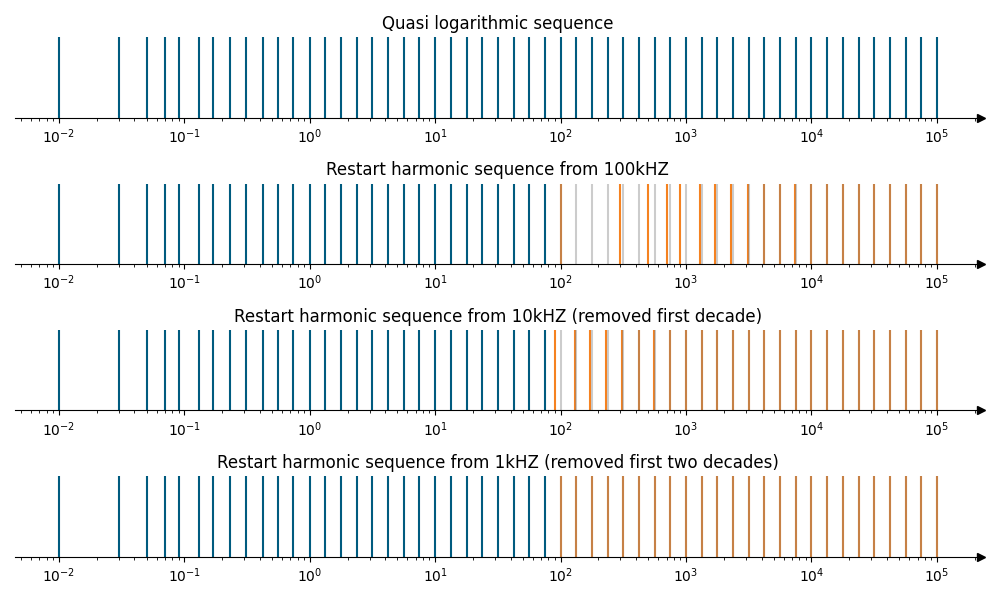
\includegraphics[width=1\linewidth]{figures/harmonics_supporting.png}
    \caption{Enter Caption}
    \label{fig:splitting_design}
\end{figure}

To summarize, for a CCCV experiment for batteries, on channel of the generator would have loaded in memory two low band multisine waves, one optimized for chronoamperometry and the other from chronopotentiometry, and the other channel have loaded the two optimized high band mutisine waves.

The automatic switch of the multisine during electrochemical experiments as described before can still be done by DEISchannel for the case of combined multisine waves passing during initialization the object MultisineWaveCombined, also provided  in the package TrueFormAWG.

\section{Automation of the acquisition for batteries}

The potentiostat is used only for the electric control of the cell while not applying any perturbation while the waveform generator provides the multi-frequency excitation as well as the quasi-cyclic voltammetry pattern. 
The arbitrary waveforms are loaded manually to the device via a .arb file transferred via USB drive from the computer. How the .arb file is build?
This approach was the one I used for the first two applications (topic of the third and final part of the thesis) of the dynamic impedance for energy storage, also published as peer-review articles.

For the goal of the thesis of acquiring the dynamic impedance during the CCCV cycling of a battery the previously described approach is not enough. 
Two problems arise: the first is the huge amount of data streamed from the device to the computer to be saved into the RAM, limited to a few GB, and secondly the need to change the waveform for the excitation  during constant current (chronopotentiometry) or constant voltage (chronoamperometry) steps. 
To overcome this problem and automation routine is needed, but before going into it I shall unpack the two issues one at the time. 
Recarding the managment of the streamed signals the problem is to sample for a long time, in the scale of weeks or months, while acquiring at high frequency. 
Let's say that one choses a moderate sampling frequency of 50kHz while sampling a system escited with a miximum frequency of 10kHz, it means 50kSa per second are stored, equivalent to 355 MSa per hour that we can translate to about 4.3 GB per channel per hour. 
Even using systems with huge memory, only a few hours of acquisition would be possible, not weeks. 
The alternative is to store into the hard drive the sampled signlas before the RAM is filled up and without loss. 
One can decide a fixed ammount of points for the storage or execute the saving at the end of a technique (chronopotentiometry or chronoamperometry). 
Before commenting which of the two approaches are more suitable for the project, I must discuss the second of the issues mentioned above. 
The multisine, its design will be throughly eplained in a later chapter, is not just characterized by the frquency content but also its absolute and the relative amplitude of the sinusoidal components. 
The absolute amplitude is important for making the experiment itself, in the sense that for a chronoamperometry experiment the amplitude in volt of the excitation is the exact value applied on the cell. 
For a chronopotentiometry experiment instead, the signal in volt prodiced by the generator is converted to current passing though the measurement resistor. 
It is clear that the amplitude of the excitation must be changed when the running technique is a chronoamperometry or a chronopotentiometry. 
In addition, the relative amplitudes of the single sinusoidal components must be optimized (instead of being all equal) to the system. 
The method I prefer to use is to measure the impedance once experimentally and deduce its module to decide the relative amplitude of each sinusodial component such that the output has a certain amplitude for a good signal to noise ratio. 
In other words, if one follows the formula

$$
V_{output}(\omega _i) = |Z_{exp}(\omega _i)| \times I_{input}(\omega _i)
$$

can deduce the necessary current to obtain a certain oscillation in volt for each sinusodial component for the system under study. 
It is foundamental to note that the relative amplitude for a chronoamperometry experiment would be the rexiprocal of the one for a chronopotentiometry techinque to maintain the same signal to noise ratio. 
For this reason one should generate two different multisine with the two series of relative amplitude and then generate them during the correct technique using a suitable total multisine amplitude to perturb the system enough. 
It is indeed an art that require trail and error and a lot of time spent on looking at the peaks of the Discrete Fourier Transform for input and otuput.









\subsection{Software solution}

The work around for both the questions seems to be an automatic system that can, during the execution of the experiment, changed the excitation in the waveform generator remotely accordignly to the technique in execution and save the signals from the scope when a technique is finished. 
This simple idea hides the main technical complication of this work: having a computer program that workd with the generator and scope, and also monitors the execution of the sequence of techniques that forms an CCCV experiment.
The software that BioLogic provides EC-Lab is not ment for software automatino but can only send trigger analog signals to other device. 
It would solve the communication with the generator but not with the streaming software of the scope. 
Luckily, BioLogic do provide the API for the control of the instruments in multiple programming languages, including Python. 
The downside is that the API is not officially supported and it is vary primitive. 
Especially the data has to be streamed from the machine and converted manually in the user code, similarly to the code for the scope. 
So I decided to write a library for the control of the BioLogic workstation in Python with some specific requirements:
\begin{itemize}
    \item work in multi-threaded fashion to allow multiple channels from the same machine to work independently and each of them to communicate to the device without blocking execution;
    \item allow easy integration with other libraries to create flexible set-up;
    \item allow to construct the same experiment structure, i.e. sequence of technqiues, of EC-Lab to compare results from both.
    \item implement software limits for voltage and current that consider the average value of the quantity to compensate the oscillation of the multisine.
\end{itemize}

\subsection{Design principle}

The automation of the instruments compatible with multi-threading uses the design pattern of the worker object. 
A worker object execute operation inside a \emph{while True} block on a dedicated thread, and terminates with a pause of 1 second of less (with the sleep command) during which the main thread is allowed to execute the code of another worker object. 
The multi-threading standard library of Python is capable of automatically manage all the objects without user indication in the code (compare to the other library like asyncio).

Worker object has a propriety with the name \emph{running} that can be used from other object to check their status. 
This idea is at the base of all the library used to syncronize the electrochemical workstation, waveform generator and scope. 
It is important to notice that given the modularity of the apporach, it is possible to use different hardware to perform the experiment in the same manner, given the interface is similar (i.e. it has the same name of the methods that return the same objects).

% Multi-threaded objects can share memory in the form of memory buffer to avoid the well known problem of concurrency. Since all the mathematical operation in the Python code uses the library Numpy and its array type for storing the data it made sense to me to have a circular buffer with the type of Numpy array to work with. Unfortunately the only existing implementation on public repositories (NpCircularBuffer) was not updated to the current version of Numpy, therefore I made and published my own simple implementation of a one-dimensional circular buffer with the name npbuffer and used it across the library needed for this project.

\section{DEIStools: a Python application for dynamic impedance}
% Clear, but needs a structural explanation before diving into components.
% Use a block diagram (even ASCII) to anchor the explanation.
% Avoid too much focus on worker objects — describe functionality.
The previous sections introduced the ideas of automating the multi-sine switch, save acquired signals periodically and process the signals online. 
These tasks are performed for each of the active channel of a multichannel electrochemical workstation. The hart of the operation is a library with the name DEIStools that contains everything need to prepare the experiment, execute it, analyses the data and visualize the results.
It builds upon the separate libraries that interface with the three devices of the set-up using the same \emph{worker object} building block discussed before.
DEIStools provides the object DEISchannel that automate the measurement. 
The user provide to the class initialization the objects for the Channel of the electrochemical workstation, the generator and the scope, already connected and initialized. 
For the online processing of the signals, another object is provided by DEIStools called PicoCalculator, that has the name suggest, takes the PicoScope object and extend its functionality to perform the calculations on a block of data of a specific length (one can think of the concept of windowing of signal processing). 
To continue into the idea of modularity, the calculation is performed by the object BlockCalculator that receives as arguments of its method a numerically converted copy of the signals (from the ADC values), and performs with them the FFT-EIS and downsampling.
With this design, the processing can be personalized for new experiment without touching the rest of the code for automation. The calculation is, as well, performed on a dedicated thread while the PicoScope object keep receiving data from the device without interruption.

Finally, the sequence of multisine waveforms, their amplitude, sampling frequency and when to turn them on in the sequence of the experimetn is also managed by a convenient object MultisineWave that the user passes to DEISchannel.
The modularity is provided by the software design pattern of dependency injection. The object Channel of pyeclab, for the control of a workstation channel accept as attribute a function that is always execute at the end of a technique, that, for the case of DEISchannel, executes the saving of the downsampled signals and updates the multisine.

\subsection{Software limits}

When a multisine is applyed on top of the drift, it is difficult to determine when to stop the galvanostatic experiment. 
Generally batteries are cycled between an upper and lower voltage limit and the constant voltage step of the CCCV terminated on a lower limit for the current. 
The easiest approach is to add to the desired limit the amplitude of the oscillation, but this is not always known. 
In my approach, I implemented two options for avarage limits. 
One is included in the DEISchannel object and computes the average over a user-selected number of points from the sampling of the workstation (note: not the scope, so the signal is likely to contain strong aliasing). 
The other is performed by the PicoCalculator object that uses the value of the zero-frequency bin in the DFT already calculated for the processing of the data, sparing any further computation. In both cases, the user can specify as many software limits as desired, using the proper syntax.


\section{Data and metadata saving}
FAIR data are essential for makeing the diffusion of DEIS possible.

% \section{The computation of impedance for non-stationary systems}
% %Under which conditions the system can be approximated as locally LTI
% %Over what window the drift is negligible
% %Why the multisine period must be shorter than the drift timescale

% \section{Online processing and data reduction} 
% \label{On-line computation}
% % This is central and should be highlighted earlier.
% % Add a conceptual figure
% The automation of the acquisition allow to record signals for battery cycling and mixed techniques but still has on other limitation regarding the data size. When considering the impedance of a battery, the desired frequency range might differ depending on the chemistry. In some cases 100Hz could be the maximum needed frequency for bigger batteries in pouch format, but when going to smaller sizes and laboratory scales it is generally needed to probe until higher frequency, up to 1MHz where the inductance of the connections cell to instrument became the predominant response (here I am not including solid state electrolytes that might need frequencies up to 7 MHz). For the application presented later, I determined an highest frequency of excitation of 100kHz (maintaining the lowest to 10mHz) that requires a sampling frequency of 500kHz or 1MHz (both worked in my tests using the following method, although according to the Nyquist limit 250kHz is enough). Such an high sampling rate would store very big data in the hard drive that soon will require expansion after weeks of measurement and experiment repetiotion. Furthermore the highest frequency would be repeated for a huge amount of times while we are actually interested of sampling long times to identify the lowest frequency. The upper part of the frequency band can be considered in a quasi-stationary condition and therefor doesn't require mathematical techniques to decouple with the main drift. The method used here follow this idea: calculating the impedance of the upper part of the frequency band (ex. above 10Hz) using the FFT-EIS method, apply a low-pass filter to remove these same frequencies and decimate the signal to a much lower rate (ex. 50Hz) to be stored for later estimation of the time-varying impedance (ex. with DMFA). Finally, the total spectra is reconstructed concatenating the impedance estimated with the two methods.

% This is the first contribution of this work: measuring broad-band non-stationary impedance continuously during the cycling of the battery.


% \section{Impedance estimation}
% % Good technical detail, but DMFA theory is misplaced.
% % Move DMFA theory to the identification chapter, keep practical aspects here.
% In the experimental works presented in this thesis, we estimated the impedance using the methods of the sliding short-time Fourier transform and dynamic multifrequency analysis; the first only during the online signal processing. The STFFT method has not much tuning. The only user parameters are the length of the window and the windowing function type. The length is dictated by the resolution that one wants to achieve, so on the lowest frequency component of the excitation. The windowing function instead alters the input and output signals time series to put more or less importance to the central part of the signal rather than the borders (makes the impedance confined in time at the price of spectral power) to obtain the instantaneous impedance at the middle points. For the experiment presented here, I assumed that being the drift of the system much slower than the perturbation, the impedance would not vary much and no windowing function is necessary. For the Dynamic Multi-Frequency Analysis, one needs to chose a filter function with care. Here we used the symmetric Fermi-Dirac delta with bandwidth of 0.01 Hz and an order of 8. A previous publication of the group showed the effect of these two parameters on the final result. The most important is the bandwidth because it reflects on the number of spectra estimated and their separation in time. Battistel and al. showed in XX the shape of the filter function when trasnformed to the time domain and it is similar to a sinc function for its main lobe and small oscillation asintothycally to zero. The dynamic multifrequency analysis performes a multiplication in the frequency domain  of the filter with the fourier spectra of the signal around one frequency, that correspond to a convolution of the time domain. Hence the time-domain transformed filter as a function shifted in time by a quantity equal to the reciprocal of the bandwidth. The windows should not be shorter than the period of the multisine and furthermore one should put care in the oscillating lobes that could bias the impedance estimation, as shown in Chukwu.

% In both methods, one can strongly reduce the zero-frequency skirt in the Fourier space and the Gibbs effect  by removing the baseline for current and voltage signals. I chose to use just a simple baseline removing because other classical methods did not work for me. Typically one can use sliding window averaging, spline or polynomial fitting or gaussian process regression to name the main one. In my experience non of these methods could effectively decouple the trend and the first few frequencies of the multisine that are overlapping. A complete Python library can be used to test these and more trend removal techniques, it is called Wotan. Hellemans and al. developed a method for de-trending signals with low frequency containing multi-sine but there is no available Python implementation to try out and the functional analysis used in the official is above my mathematical skills to implementing it myself.

% \section{Consideration on the drift}
% % Why using quasi cyclic voltammetry.

\section{Limitations and future improvements}
% Expensive hardware, could be streamlined
% Clock synchronization of generator and sampler
% Better optimization of the multisine
\chapter{Interpretation of impedance}
\label{chap:analysis}
% \minitoc

\section{Parametric models}
Once the impedance is measured, one can attempt to identify its dynamic fitting a physical or non-physical mathematical model (parametric). The work presented later in this work use one type or the other. The physical models where all taken from the literature. We used a model for ion adsorbtin on nanoparticle to analyse the measurement of electrical double layer capacitors and we adapted a model for intercalation with porous electrode theory both developed inside the group in the previous years. The core measurement of this work was made on lithium-ion cells, that is not the classic analytical cell with reference electrode commonly emplyed by electrochemists. The absence of the reference electrode makes cumbersome to develop a physically derived model so we decided to take the route of black-box model. Compared to the time-domain characterization where plenty of black-box models exist for any type of systems (ARMA, ARIMA, NARMAX, ecc.), the frequency-domain characterization lacks such variety and standardization, especially for time-varying systems. The approach in our group is to estimate the instantaneous impedance at quasi-stationary points using the dynamic multi-frequency analysis, hence treating the system as linear and time-invariant. Therefore the approach is to fit a generic rational function of order n infering the correct structure of the transfer function of the system though statistical methods. 

\subsection{Physical model for intercalation in porous electrodes}

The impedance of intercalation materials is modeled using porous electrode theory, originally developed by De Levie for porous metal electrodes and later adapted by Bisquert and others for insertion battery materials. The model accounts for both the ionic transport through the electrolyte-filled pores and the charge transfer/intercalation processes at the electrode-electrolyte interface.

\subsubsection{Theoretical framework}

For a porous electrode, the impedance can be derived from a transmission line model where the electrode is represented as a series of parallel resistor-capacitor elements along the pore depth. The total impedance combines:

\begin{itemize}
\item \textbf{Electrolyte resistance in pores} ($R_e$): ionic transport resistance through the liquid-filled porosity
\item \textbf{Charge transfer resistance} ($R_{ct}$): resistance to ion insertion/extraction at the particle-electrolyte interface
\item \textbf{Double-layer capacitance} ($C_{dl}$): capacitance of the electrical double layer at the interface
\item \textbf{Chemical capacitance} ($C_\mu$): capacitance associated with the change in chemical potential during intercalation
\item \textbf{Diffusion impedance} ($Z_D$): solid-state diffusion of intercalated ions within particles
\end{itemize}

For a porous electrode with cylindrical pores of length $l$ and distributed impedance per unit length, the total impedance follows:

\[
Z(\omega) = \sqrt{Z_0 \cdot Z_L} \coth\left(\sqrt{\frac{Z_L}{Z_0}}\right)
\]

where $Z_0$ is the electrolyte resistance per unit length and $Z_L$ is the interfacial impedance per unit length, given by:

\[
Z_L = \frac{1}{j\omega C_{dl} + \frac{1}{R_{ct} + Z_D}}
\]

The solid-state diffusion impedance for spherical particles of radius $r_0$ follows:

\[
Z_D = \frac{R_{ct}}{j\omega \tau_D} \coth\sqrt{j\omega \tau_D}
\]

where $\tau_D = r_0^2/D$ is the characteristic diffusion time and $D$ is the chemical diffusion coefficient.

\section{Physical model for intercalation}

% Take it from the paper

In order to interpret the dynamic spectra, we used a physically-based porous electrode model derived from a simplified transmission-line approach. It accounts for ionic transport in the electrolyte-filled pores, electron conduction in the active material, and Faradaic intercalation kinetics. The overall impedance is represented as:

\begin{equation*}
Z_T = R_s + \frac{R_p}{k l} \coth(k l),
\end{equation*}

where $R_s$ is the uncompensated solution resistance, $R_p$ combines pore-solution and solid-particle resistances, and $kl$ embeds the finite diffusion or charge-transfer response of the porous electrode. This approach has been discussed in \cite{scarpioniElectrochemicalImpedanceSpectroscopy2023a} and references therein.

\begin{figure}[H]
    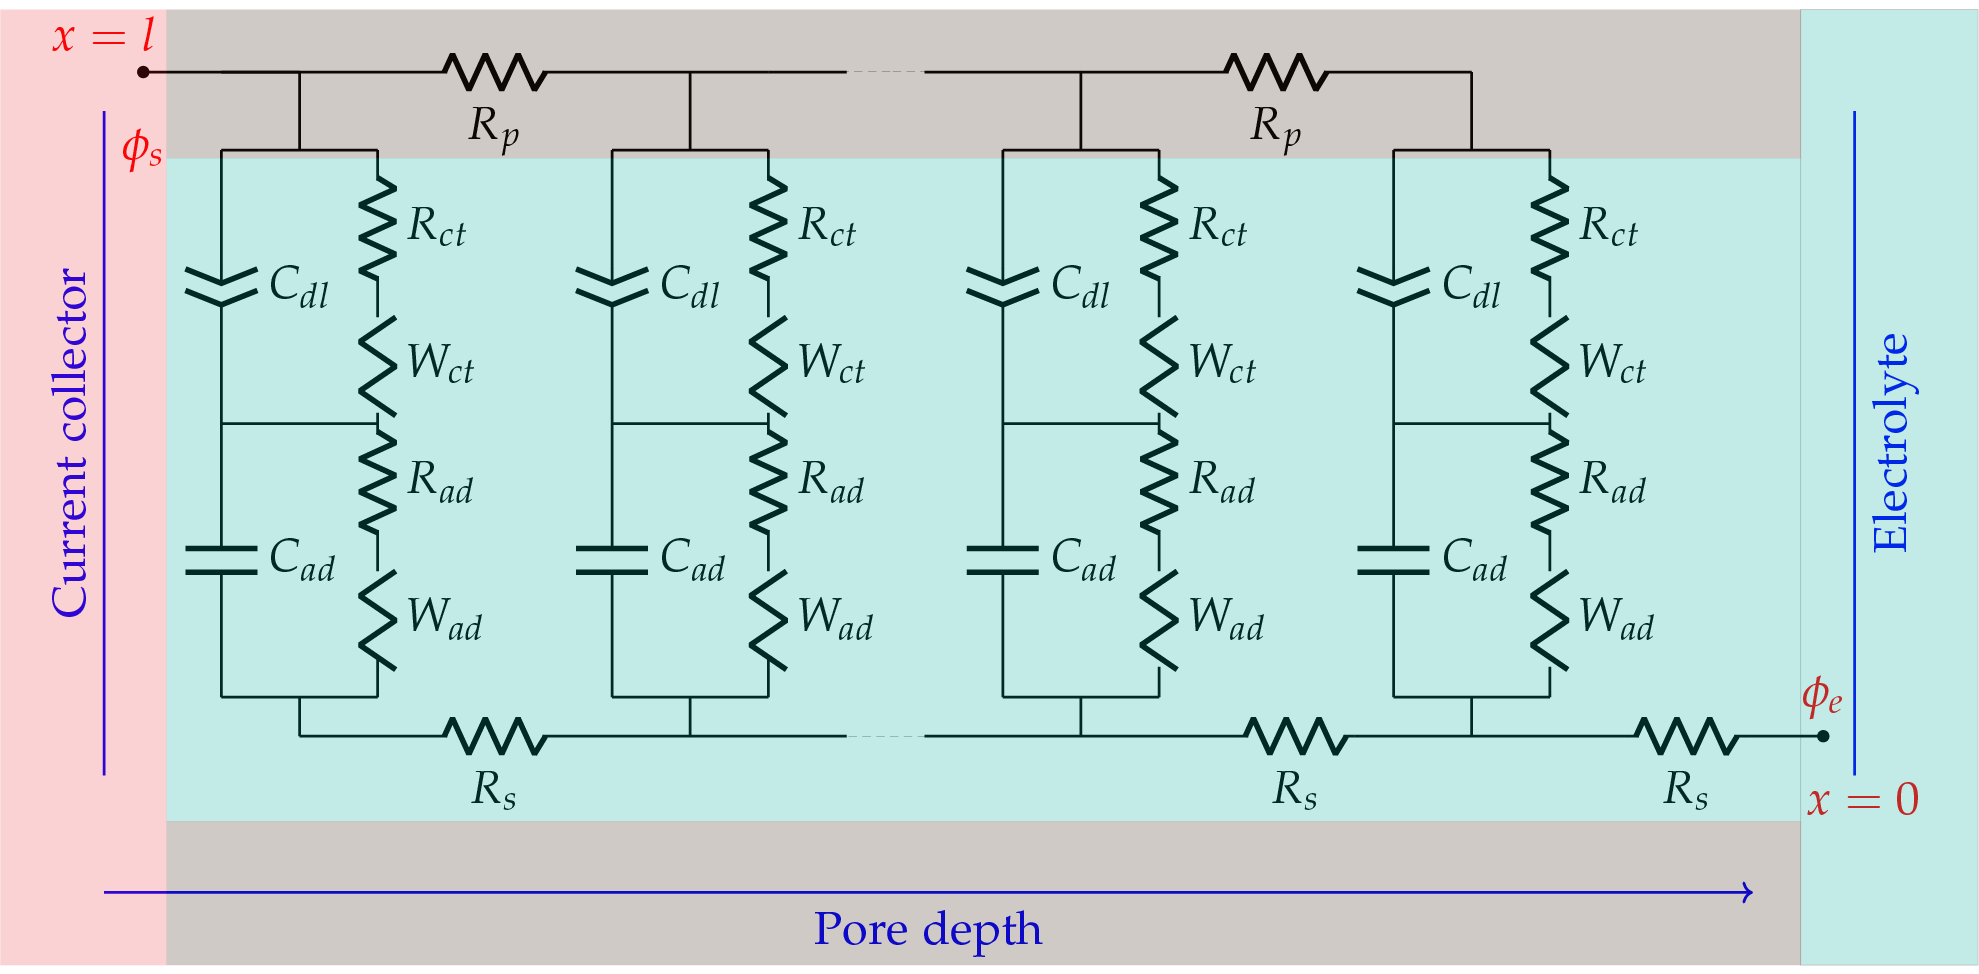
\includegraphics[width=\textwidth]{figures/LTP/ltp_circuit_new.png}
    \label{fig:LTP circuit}
    \caption{Equivalent circuit of the physical model used to fit DEIS spectra.}
\end{figure}

The interface processes are described by the following simplified unit (Figure \ref{fig:LTP circuit simplified}) in the transmission line where the Warburg element rapresenting the charge trasnfer has been substituteby a capacitor. This semplification produces better fit with lower ammount of paramters.

\begin{figure}[h!]
    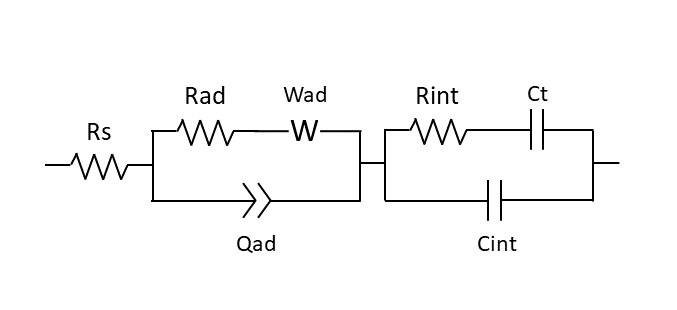
\includegraphics[width=0.8\textwidth]{figures/LTP/EC_collins_simplified.jpg}
    \caption{Equivalent circuit of the physical model developed for the intercalation processes of MnO2 in \cite{erinmwingbovoDynamicImpedanceSpectroscopy2020}}
    \label{fig:LTP circuit simplified}
\end{figure}


\subsubsection{Simplified model for time-varying impedance}

For the dynamic impedance measurements presented in this work (Chapters 10-11), a simplified version of this model was employed. At frequencies above the diffusion regime but below where inductive effects dominate, the impedance can be approximated by:

\[
Z(\omega) = R_s + \frac{R_{pore}}{\sqrt{1 + j\omega\tau_{pore}}} + \frac{R_{ct}}{1 + j\omega R_{ct}(C_{dl} + C_\mu)}
\]

where:
\begin{itemize}
\item $R_s$ is the solution resistance (ohmic drop)
\item $R_{pore}$ captures the distributed pore resistance
\item $\tau_{pore} = R_e C_{dl}$ is the characteristic pore time constant
\item The third term represents the charge transfer process coupled with both double-layer and chemical capacitance
\end{itemize}

This form yields a characteristic impedance spectrum with:
\begin{enumerate}
\item A high-frequency intercept corresponding to $R_s$
\item A depressed semicircle in the mid-frequency range from the porous electrode behavior
\item A second semicircle or Warburg-like tail at low frequencies from charge transfer and diffusion
\end{enumerate}

\subsubsection{Application to lithium titanium phosphate}

For the LiTi$_2$(PO$_4$)$_3$ electrodes studied in Chapter 10, this model was fitted to dynamic impedance data acquired during both galvanostatic and voltammetric perturbations in aqueous sodium-ion electrolyte. The key findings were:

\begin{itemize}
\item $R_{ct}$ varies significantly with state of charge, reflecting the potential-dependent kinetics of Na$^+$ insertion
\item An asymmetry was observed between charge and discharge, attributed to differences in solvation/desolvation activation energies
\item The porous electrode contribution ($R_{pore}$) remained relatively constant, confirming good ionic connectivity throughout cycling
\item Chemical capacitance $C_\mu$ peaks near 50\% state of charge, consistent with the voltage plateau region where the thermodynamic factor $\partial \mu / \partial c$ is maximized
\end{itemize}

This physical interpretation was only possible due to the use of a three-electrode configuration with a properly positioned reference electrode, enabling separation of the working electrode impedance from the counter electrode contribution.

\subsubsection{Model for electrical double-layer capacitors}

For the symmetric activated carbon electrodes (Chapter 11), a similar porous electrode framework applies, but without the Faradaic charge transfer term. The impedance simplifies to:

\[
Z(\omega) = R_s + \frac{R_{pore}}{\sqrt{1 + j\omega\tau_{pore}}} + \frac{1}{j\omega C_{dl,eff}}
\]

where $C_{dl,eff}$ is the effective double-layer capacitance of the porous structure. The model accounts for:

\begin{itemize}
\item Ion adsorption/desorption at the carbon surface (non-Faradaic process)
\item Distributed ionic resistance within the nanoporous carbon network
\item Frequency dispersion due to pore size distribution (often modeled with constant phase elements)
\end{itemize}

Despite using chemically identical electrodes, the positive and negative electrodes exhibited different impedance magnitudes and time constants during cycling, attributed to:
\begin{enumerate}
\item Different electrochemical histories (voltage excursions)
\item Adsorption of electrochemically inactive species (e.g., oxygen reduction products at positive electrode)
\item Asymmetric ion accessibility at different potentials
\end{enumerate}

The time-varying impedance revealed that these effects evolve continuously during charge/discharge, information that would be invisible in traditional equilibrium measurements.

% \section{Simultaneous fitting}

% The approach of fitting for dynamic impedance is similar to what is commonly done for static impedance, but there is the challenge that for a non-stationary experiment the dynamic of the system can change with the activation or deactivation of chemical processes with time, voltage or temperature. For example, a battery would change its state of charge during a galvanostatic technique and the system response might change at different potential, and with its cycling history.  The common approach, sometimes called batch fitting, would be of fitting one spectra of the time using the optimized parameters of the previous spectra for the following. The problem is that some parameter of the model would be close to zero in some part of the dataset and potentially very big in others. Solving optimization problems with small and redundant parameters might lead to local solutions. Furthermore, when more than one parameter is of this type, the solver might converge to different minimum for each spectra even when the optimized parameters of the prevoious spectra are used as starting points. This issue can be addressed minimizing the entire dataset at ones and introducing a regularization term in the objective function as firstly introduced by Battistel et al. The objective function become: \\

% equation?\\

% Intuitively, one can consider a term that minimizes the distance between data points and model while another term keeps the parameters slowly evolving across the dataset. The penalty term avoids sudden variation of parameters that arises in those areas of the dataset where there is unavoidable overparametrization.
% Recently Cuckwu extended the concept of  penalized objective function implementing modern methods to solve high dimensional optimization problem as used in the field of Machine Learning. An improvement in computation time for big dataset has been obtained combining the efficient methods for calculating derivatives called "automatic gradient" or automatic differentiation and the solver ADAM. Both can be find in the open source package JAX that uses the Python pre-compiling from the jit library to perform the calculation in multiple threads, processors or even distributed computing (including GPUs). JAX is supported for optimization-specific problems in the open source package Optax. Cuckwu implementation is open source but compatible up to Python 3.9 and only with JAXopt, the previous project from which Optax derived (not in development anymore). Dr. Nicoló Pianta updated Chucwu's code base to modern version and added a convenient object rapresentation for the model function, similar to the well-enstablished python library for non linear fitting nlfit. For each experiment of the Applications part I will specify which library was used to analyze the impedance.\\

\subsection{Fitting error}
We estimate the standard deviation from the Jacobian of the objective function. The error allows to verify in most of the cases the accuracy of the model and which parameters are not significant in the estimation.

\section{Determination of the system degrees of freedom}

When fitting physical models, the user decides \emph{a priori} the degreese of freedom of the system though the number and types of approximation and the equation that chose to keep. The process of model regression gives to the scientist a confirmation that the model can represent the nature of the system under the operating condition or not. On negative result one keeps modifying the model until satisfied. On the other hand, when working with black-box model the scientist makes the opposite: identifies the degreese of freadom of the system and then look for a proper gray-box or white-box model of the same structure to undenstand the physics of the system.  This data driven apporach relies on the fact that the frequency reponse function is a numerical realization of the real transfer function of the system inside the frequency band of the experiment. From dynamic system theory it is known that the number of parameters of the transfer function is equal to the number of variables in the state space model, directly connected to the differential equations that define the system. For batteries, that works as two-electrode devices, the response of the single electrode is superimposed making even harder to define a general physical model. Usually the model are largely over-parametrized. Knowing the correct transfer function, leads scientists to chose proper approximation when developing physical model or can be is as it for prediction or classification of the system in control engeneering. It immediatly come to mind the possibililty of using it for smart control of the battery in battery managment systems. 

\section{Determining transfer function structure}
The identification of the transfer function structure is the process of finding the order of the nominator and denominator of the polynomial rational function through statistical approach. In this work I ... 

\part{Results and discussions}
\chapter{Coin cells: characterization at the cell level}
\label{chap:coins}

% Objectives
In this chapter, I present measurements of dynamic impedance on commercial batteries during operation. 
The aim is to demonstrate the applicability of the mixed method for instantaneous impedance estimation under non-stationary conditions.

I chose to conduct this experiment on commercial coin cells with a theoretical capacity of 45 mAh because of the convenience and low cost of purchasing large quantities. 
I acquired a set of identical commercial coin cells and tested them using the dynamic impedance method during cycling, alongside conventional electrochemical measurements for comparison. 
The results from the dynamic impedance experiment are compared with a series of classical stationary impedance spectroscopy measurements. 
\marginpar{
  \centering
  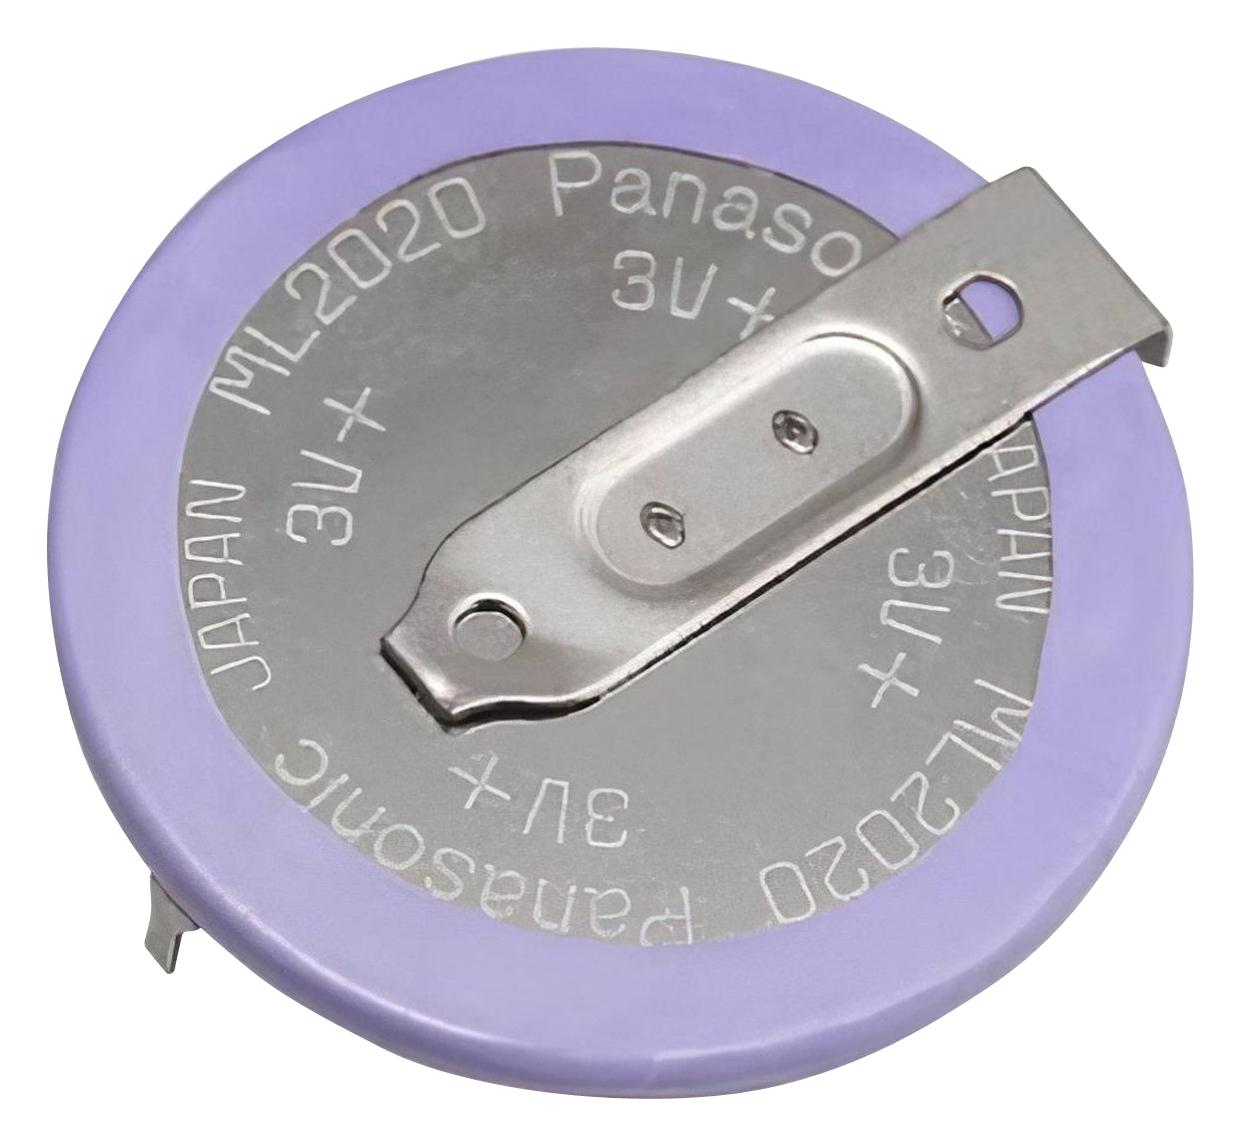
\includegraphics[width=0.5\marginparwidth]{figures/results_coin/panasonic_ML2020_photo.jpg}
  \captionof{figure}{Panasonic ML2020 coin cell format battery used to test long-term cycling with dynamic impedance spectroscopy.}
  \label{fig:coin cell}
}
Furthermore, I demonstrate that the presence of a multi-sine perturbation continuously applied during the dynamic impedance spectroscopy test does not affect cell aging.

% Summary of experiments
This study comprises the following measurements:
\begin{table}[h]
\begin{tabular}{ccc}
\toprule
Measurement type & Number of cells & Number of cycles  \\
\midrule
DEIS during CC-CV & 9 & 30\\
Traditional CC-CV& 12& 22--30\\
EIS during interrupted CC-CV & 3& 1 \\
\bottomrule
\end{tabular}
\end{table}

\section{Experimentals}

\subsection{Cell choice}
% Cell chemistry and implications
For this research, I acquired a set of identical Panasonic ML2020 coin cell batteries containing manganese dioxide (MnO$_2$) as the positive electrode and a lithium--aluminum alloy as the negative electrode. 
The lithium content is approximately 0.02~g. 
These cells utilize an electrolyte solution composed of 1,2-dimethoxyethane and ethylene glycol dimethyl ether (EGDME) combined with an unspecified lithium salt.

According to manufacturer specifications, these batteries have a nominal capacity of 45~mAh and are designed to operate within a voltage window of 1--3~V, with a recommended charging current of 100~$\mu$A. 

The cells exhibit relatively slow kinetics compared to NMC/graphite systems due to the viscosity of the electrolyte, and they experience rapid capacity fade---a characteristic of low-power designs at modest C-rates. 
They are designed as buffers for low-power electronics; thus, a viscous solvent is used as the electrolyte to reduce self-discharge.
When cycling at a C-rate of C/10, the cells degrade rapidly, reaching end-of-life in approximately 22 cycles, with short-circuits often observed. 
I attribute this to lithium plating in dendritic form.

These limitations are actually favorable for rapidly iterating optimizations of the set-up.
The use of commercial cells ensures reproducibility for validation of the method. 

\subsection{Dynamic impedance spectroscopy measurements}

\subsubsection{Setup description}
% \marginpar{
%   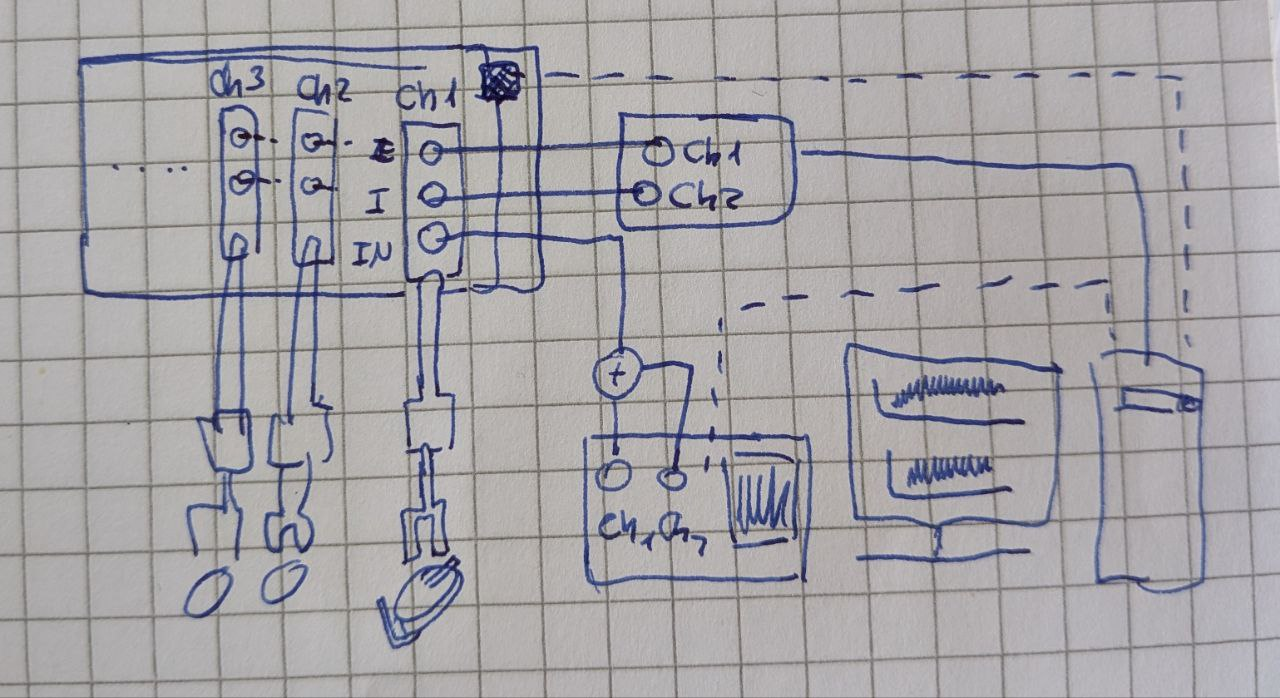
\includegraphics[width = 0.8\marginparwidth]{figures/results_coin/sketch_DEIS_setup_new.jpg}
%   \label{fig:DEIS setup coins}
% }
I conducted the measurements of this chapter using the setup configured for broadband multi-sine waves: two channels of the generator apply two multi-sine excitations covering a total of 7 frequency decades, and the computer processes the streamed data from the oscilloscope in real time as described in Section~\ref{On-line computation}. 
Three of the six channels of the BioLogic SP-300 potentiostat were measured simultaneously thanks to the multi-threading capability of the software \verb|EIStools|. 
% The connection of the instruments is shown in Figure~\ref{fig:DEIS setup coins}.

\subsubsection{Multi-sine design}
The multi-sine waveform excitation contains 49 frequency components in the range 10~mHz--100~kHz, generated at 250~kSa/s, thus one period is of 100~s. 
The total waveform is split into two parts as described in Section~\ref{sec:multisine split} to work around the memory limitation of one generator channel. 
The amplitude of the multi-sine was optimized from a previous experiment as described in Section~\ref{sec:amplitude optim}. 

\subsubsection{Applied drift}
The potentiostat applies a constant current--constant voltage (CC-CV) sequence with an upper voltage limit of 3~V during charge and the same value for the constant voltage step with a lower current limit of 1~mA. The lower voltage limit for discharge was 1~V. The applied current was 4.5~mA, equivalent to a C-rate of C/10. Because of the multi-sine perturbation, the limits are checked during the online computation algorithm as the average value of the data block (as described in Section \ref{sec:software_limits}). The cells are cycled for 30 cycles continuously or until reaching end-of-life. 

The voltage and current signals are sampled with a two-channel PicoScope 4000 series at a sampling rate of 500 kSa/s.

After the experiment, the automated software returns the impedance of the high frequencies (10 Hz--100 kHz) computed online using the STFT method and the voltage and current signals from the cells at the reduced sampling rate of 50 Sa/s. The signals contain the lowest 21 frequency components, ranging from 10 mHz to approximately 8 Hz.

To illustrate the output of the online computation and data-reduction pipeline, Figure \ref{fig:raw_multifrequency_coin} shows the reconstructed voltage and current signals after filtering and downsampling as it is saved in the computer storage after the acquisition step.
These signals retain the low-frequency components while discarding high-frequency content already processed online.

\begin{figure}[h]
  \centering
  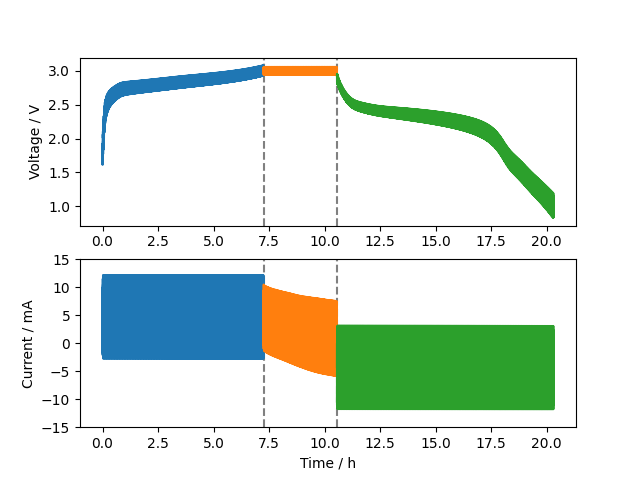
\includegraphics[width = \textwidth]{figures/results_coin/raw_data_multifrequency.png}
  \caption{Voltage and current signals sampled at 50 Sa/s after online computation and downsampling.
  The signals contain the low-frequency components (10mHz--8Hz) of the original broadband excitation, which are used for off-line DMFA estimation of the impedance and reconstruction of the electrochemical drift.}
  \label{fig:raw_multifrequency_coin}
\end{figure}

The impedance of the lower frequency band and the drift are estimated using the DMFA with a filter bandwidth of 0.01 Hz, which yields a time resolution of 100 s, equal to one period of the multi-sine and the signal block used in the online computation. The total impedance spectrum is the concatenation of the parts computed with STFT and DMFA and reported in Figure \ref{fig:dmfa_impedance_coin}.

\begin{widefigure}[!h]
  \centering
  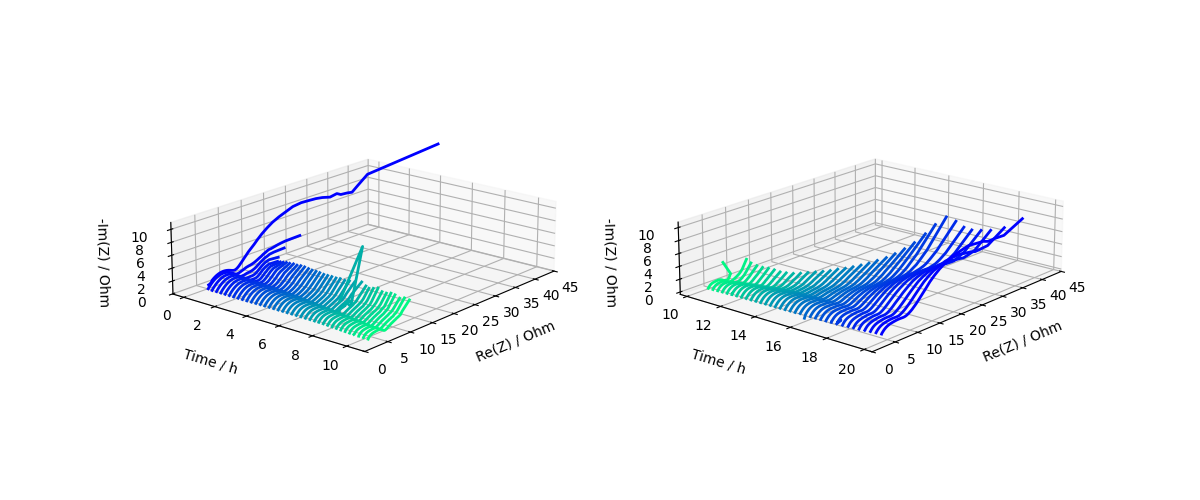
\includegraphics[width = \linewidth]{figures/results_coin/dmfa_impedance_result.png}
  \caption{Impedance of charge and discharge estimated with DMFA and online STFT combined. One spectrum per 10 cycles is plotted; the first 2 plots are discarded.}
  \label{fig:dmfa_impedance_coin}
\end{widefigure}

The effectiveness of the DMFA in separating the slow electrochemical drift from the superimposed multi-sine excitation is illustrated in Figure \ref{fig:dmfa_drift_coin}.

\begin{figure}[h]
  \centering
  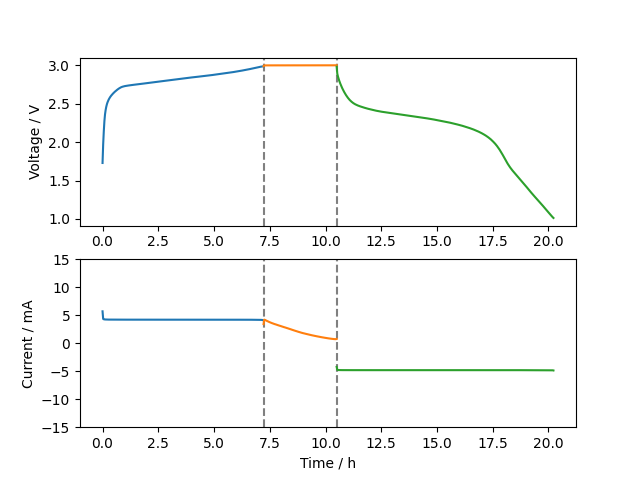
\includegraphics[width = \textwidth]{figures/results_coin/dmfa_drifts_result.png}
  \caption{Drift reconstructed using the DMFA from the downsampled voltage and current signals. The y-axis scale is kept the same as in Figure \ref{fig:raw_multifrequency_coin} for comparison.}
  \label{fig:dmfa_drift_coin}
\end{figure}

\subsection{Impedance analysis}
\subsubsection{General transfer function model}
A battery contains at least two principal interfaces (positive and negative electrodes), whose impedances are connected in series in an equivalent circuit model.
This makes it challenging to develop a physical model that effectivelly describe the system without overparametrize.

% In this work, I approached the identification problem as a black-box and used a rational polynomial function for fitting through complex nonlinear least-squares:
% \begin{equation}
%   Z (\sqrt{j\omega})= \frac{a_0 + a_1(j\omega)^{-1/2}+\cdots+a_n(j\omega)^{-n/2}}{1 + b_1(j\omega)^{-1/2}+\cdots+b_n(j\omega)^{-n/2}}.
% \end{equation}
% Setting $b_0 = 1$ prevents the function from diverging.


Instead of attempting to identify its physical parameters with a physical model (referred as a white-box model) it is equally interesting to identigy the system with a matematical model (referred as a black-box model). 
Thanks to the continous instantaneous impedance spectra generate with dynamic impedance spectroscopy, the time varaition of the mathematical model's parameters remains informative for the purpose of control and prediction. 

In this context of system identification, the battery is considered a generic linear and time-invariant system, hence the input $u(t)$ and the output $y(t)$ of a system are connected by the linear ordinary differential equation
\begin{equation}
    \sum_{N} a_n \frac{\text{d}^ny(t0)}{dt} = \sum_{M} b_m \frac{\text{d}^my(t0)}{dt}.
\end{equation}
As discussed in Section \ref{sec:laplace}, differential equation can be solved by applying the Laplace transform, which yields
\begin{equation}
    \sum_{N} a_n s^n Y(s) = \sum_{M} b_m s^m U(s),
\end{equation}
and so the transfer function for the system is given by
\begin{equation}
    G(s) = \frac{Y(s)}{U(s)}=\frac{\sum_{N} a_n s^n}{\sum_{M} b_m s^m}.
\end{equation}
This equation for the transfer function is the same of Equation \ref{eq:transfer function dy sys} from section \ref{sec:transfer function def diff equations} (p. \pageref{sec:transfer function def diff equations}).

The Laplace variable $s$ for the case of impedance is simplified to $s = j\omega$, but since the system is electrochemical, the homogeneous differential equations describing diffusion are semi-integer \cite{oldhamFractionalDifferentialEquations2010} and lead to solutions as functions of $\sqrt{j\omega}$.
Therfore for electrochemical systems the generic transfer function has the form:
\begin{equation}
    G(\sqrt{j\omega}) = \frac{\sum_{N} a_n (\sqrt{j\omega})^n}{\sum_{M} b_m (\sqrt{j\omega})^m}.
    \label{eq:general rational polynomial}
\end{equation}

In this work, I used such a rational polynomial function of order $n=m$ as a measurement model to fit impedance data.
The concept is not new \cite{zoltowskiNontraditionalApproachMeasurement2005,gheemTheoreticalApproachModelling2008a,liModelReductionFractional2024}, but it is the first time this model has been used for instantaneous impedance of time-varying systems.
Polynomial functions can flexibly fit impedance with any complex shapes and also have the advantage of working as a test for the linear Kramers-Kronig relations \cite{sadkowskiCNLSFitsKramers2004}.

\subsubsection{Regression procedure}

A fundamental procedure for the regression of rational polynomial function is to add L1 regularization to the objective function, also called LASSO (\emph{least absolute shrinkage and selection operator}).
In practice, the objective function to minimize is
\begin{equation}
  obj = \sum_n r_n^2 + \lambda ||\mathbf{\theta}||_1,
\end{equation}
where $r_n^2$ is the weighted complexed squared residual of the n-th point of the spectra as described in Section \ref{sec:fitting-sys-id}, $\mathbf{\theta}$ is the parameters array, and $\lambda$ is a penalty factor that controls the regularization strength.
Regularization is important because rational function parameters can grow unnecessarily large and be compensated by parameters in the denominator.
The choice of penalty factor is arbitrary, and I found that values as small as $1 \times 10^{-12}$ is sufficient.
Removing the regularization terms makes the optimization procedure ineffective (parameters diverge) or causes the solver to fail.


Before fitting, I removed the first three and last two spectra from the dataset, as well as the first three and last frequency points (remaining range: 30~mHz--42~kHz).

In least squares objective function introduced in Section \ref{sec:fitting-sys-id} each frequency component residue is weighted by a factor equal to the experimental error.
The error in a frequency response function increases with the lowering of the frequency.
Orazem et al.\cite{orazemEIS} originally proposed to use the inverse of the impedance modulus as weighting factor, but I found that using the square root of the modulus is more effective in this case. It weights the middle-to-high frequency range more heavily, allowing the model to fit the impedance's features better.

A better strategy would be to estimate the error from error propagation rules through elementary mathematical operations, as described in Reference \cite{chukwuStatisticalAnalysisMeasurement2022} did for admittance data estimated via DMFA.
Unfortunately, I was unable to replicate his derivation for my impedance data.
Furthermore, error propagation for the FFT impedance method is not available in the literature and must be derived from first principles.

For the optimization, I adopted a classical derivative-based approach (trust region reflective method) as implemented in the Python package \verb|LMFIT| \cite{newville_2014_11813} to solve such minimization problems.
I first fited the spectrum at the middle of the dataset using random initial parameters (seed 42) and then used the optimized parameters as the starting points for the first spectrum of the dataset. Subsequently, I proceed passing optimized parameters as initial points for the next fitting.

% Regarding the order of the rational polynomial, I chose the same order for numerator and denominator and found that 7 was the minimum order needed to represent all features with a small error.

The difficulty in fitting dynamic impedance data is identifying one set of values for polynomial order, regularization penalty factor, and least-squares weighting factor that work effectively across all electrochemical techniques in the experiment, all cycles, and are general enough to apply to multiple cells.

\subsection{Classical electrochemical test}
I performed cycling experiments using the same constant current--constant voltage protocol on a BioLogic battery cycler with 12 cells from new to aged condition to compare degradation with and without multi-sine excitation.

I also prepared an experiment performing classical electrochemical impedance spectroscopy at fixed states of charge. For this purpose, I created an experiment sequence that interrupts the cycling protocol every 10\% of the nominal capacity and includes a 1~h rest before impedance measurement in the frequency range 10~mHz--20~kHz (8~points/decade).


\section{DEIS results}

% Geometrical features across SoC (semicircles, diffusion tail, ohmic resistance) 
% and their evolution with SoH

% First cycle behavior and conditioning affects impedance

% Cell-to-cell variability and outliers

\subsection{Impedance at different battery states}

Continuous impedance acquisition provides a complete view of battery interface resistance at any state of charge and state of health. Figures~\ref{fig:deis_aging_charge} and~\ref{fig:deis_aging_discharge} show this information for charge (including the potentiostatic portion) and discharge. I compared the impedance at four states of health corresponding to the beginning, midpoint, just before the 80\% threshold of first-cycle capacity, and after it. 
It can be observed at least two consecutive semicircles and a diffusive tail. At lower states of charge, represented in red in the colored scale, a third semicircle appears, shifting the diffusion to lower frequencies.
Another observation is the change in ohmic drop resistance with state of charge.
The evolution of the impedance spectrum with battery aging during charge is summarized in Figure~\ref{fig:deis_aging_charge}.

\begin{widefigure} [h]
  \centering
  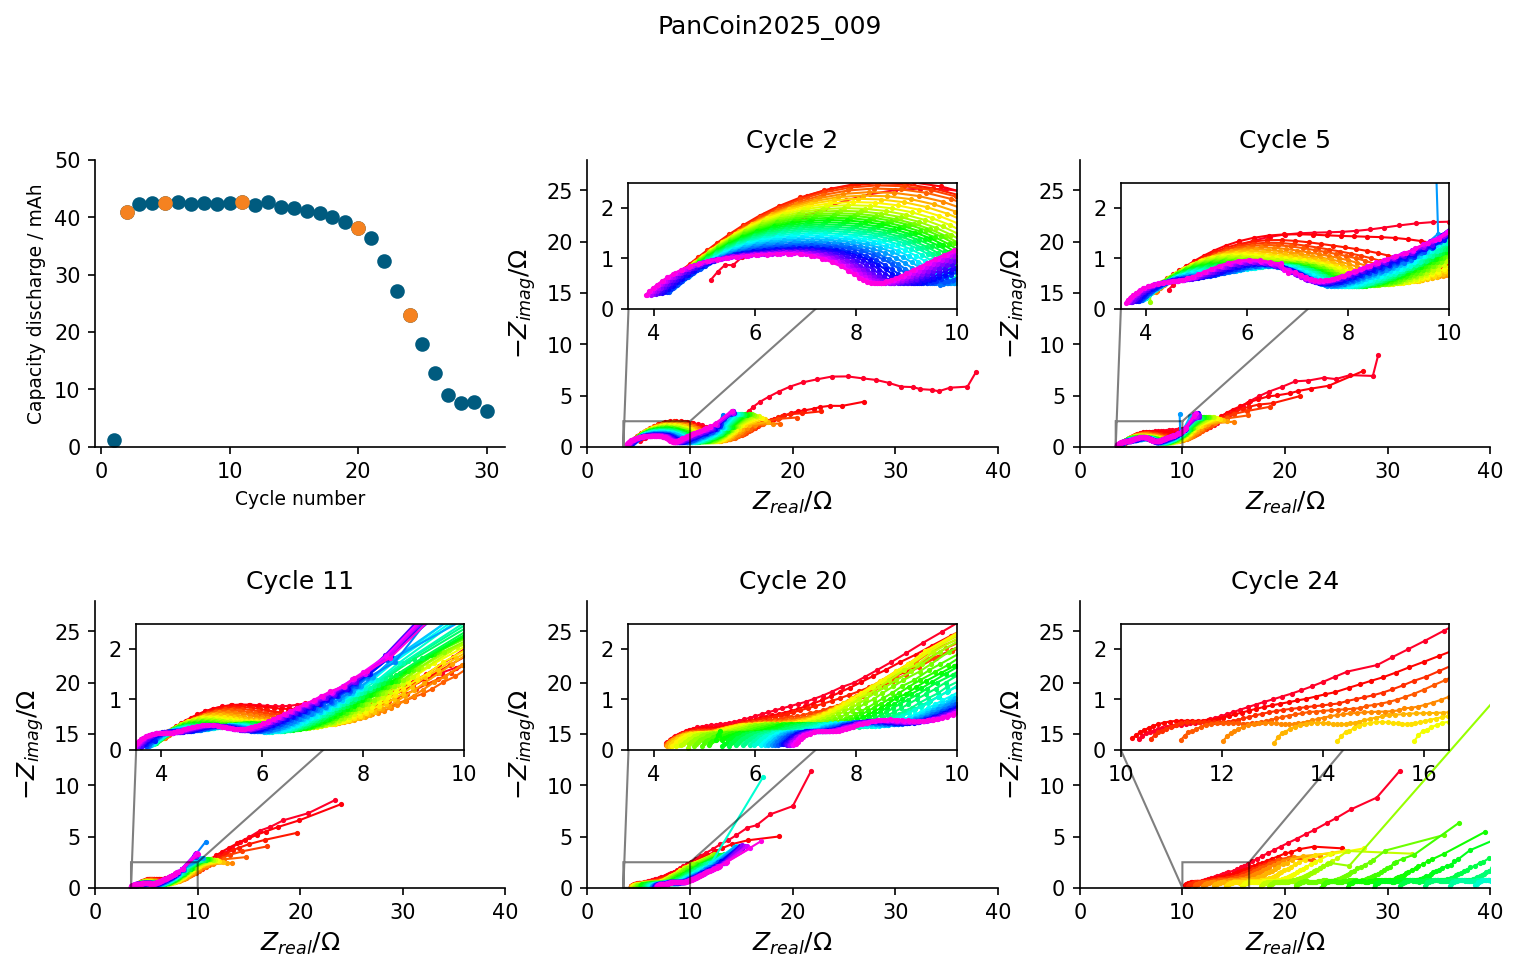
\includegraphics[width = \linewidth]{figures/results_coin/PanCoin2025_009_DEIS_charge_aging_mosaic.png}
  \caption{Dynamic impedance spectra during charge at selected states of health.
  Spectra are shown for four aging stages: beginning of life, mid-life, just before the 80\% capacity threshold, and after crossing it.
  Color coding indicates state of charge.}
  \label{fig:deis_aging_charge}
\end{widefigure}

A corresponding representation for discharge is reported in Figure~\ref{fig:deis_aging_discharge}.

\begin{widefigure} [!h]
  \centering
  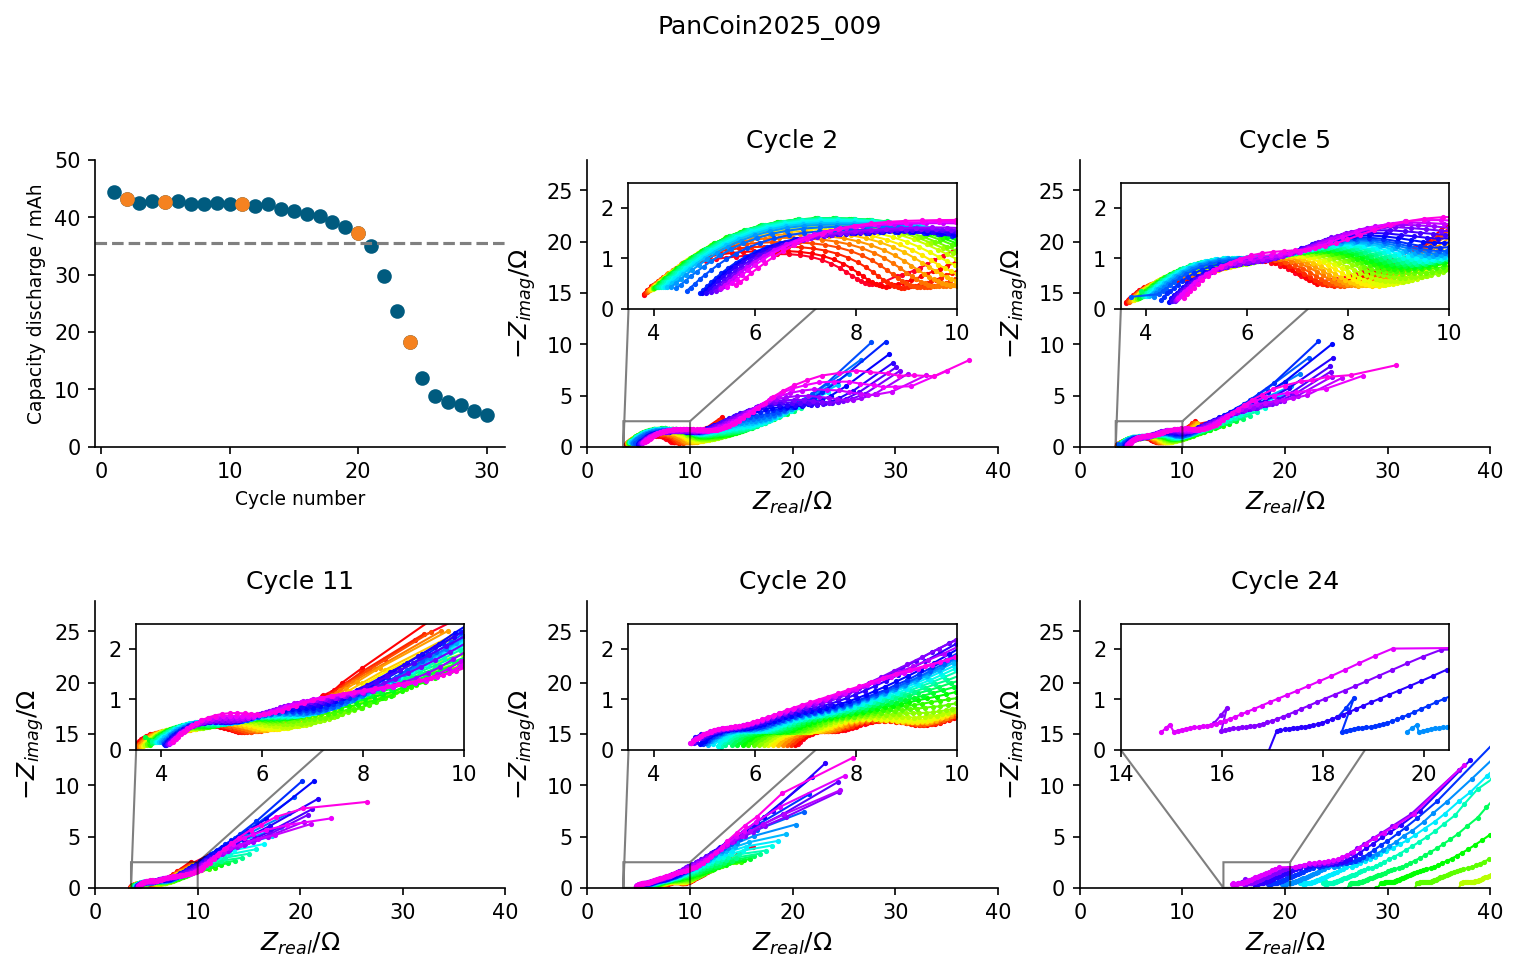
\includegraphics[width = \linewidth]{figures/results_coin/PanCoin2025_009_DEIS_discharge_aging_mosaic.png}
  \caption{Dynamic impedance spectra during discharge at the same aging stages as Figure~\ref{fig:deis_aging_charge}.
  The appearance and shift of multiple semicircles and diffusive features reflect changes in interfacial and transport processes with aging.}
  \label{fig:deis_aging_discharge}
\end{widefigure}

The cell is provided from the manifacturer at 2.75~V, so in the first cycle of the measurement, the cell voltage quickly reaches the charging limit and then precedes the discharge as shown in Figure~\ref{fig:first_cycle_coin}. 
The impedance of the first cycle is reported in Figure \ref{fig:impedance_first_cycle_coin}
% This is probably due to the state of the solid electrolyte interphase (SEI). 
% After the fir charge the SEI is damaged and freshly reformed in the next discharge. 
% I also expect some lithium deposition alongside the alloying with aluminum during the negative electrode reduction that increase the surface area exposed to the electrolyte yielding to further SEI formation.
% Looking at both impedance magnitudes, though, a reduction is noted for the cycles after the second.
% This might be connected to a thinner SEI layer.

\begin{figure} [!h]
  \centering
  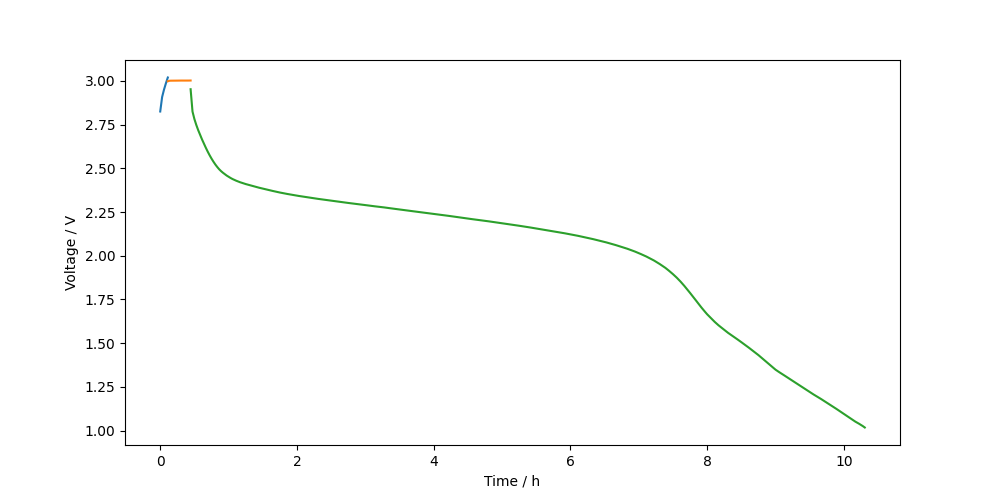
\includegraphics[width = \textwidth]{figures/results_coin/Voltage_dmfa_first_cycle_cell009.png}
  \caption{Voltage profile of the first charge--discharge cycle.
  The cell reaches the upper voltage limit early during the first charge, indicating a conditioning process that differs from subsequent cycles.}
  \label{fig:first_cycle_coin}
\end{figure}


\begin{figure} [!h]
  \centering
  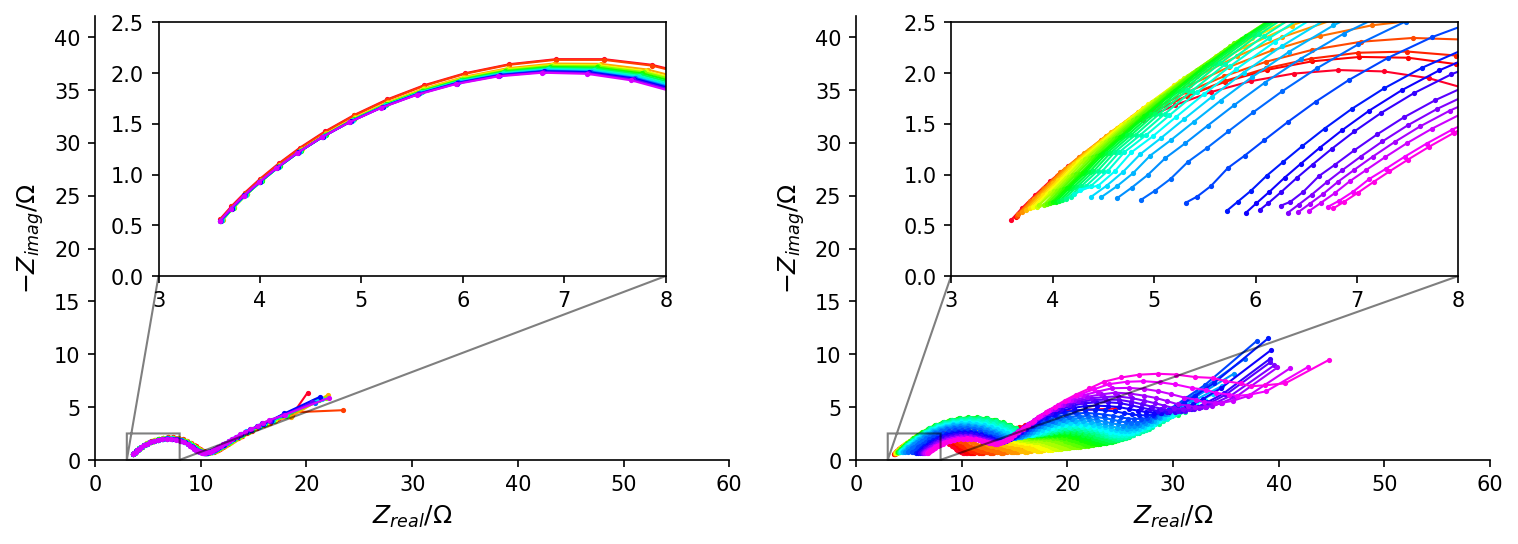
\includegraphics[width = \textwidth]{figures/results_coin/PanCoin2025_009_DEIS_first_cycle.png}
  \caption{Impedance spectra during the first cycle.
  Left: all charge spectra; right: discharge spectra with one spectrum every ten cycles.
  Both magnitude and shape differ markedly from later cycles, indicating transient interfacial processes during initial conditioning.}
  \label{fig:impedance_first_cycle_coin}
\end{figure}

All behaviors observed here are reproduced in the other 8 cells of the set, including the higher impedance in the first discharge. Detailed results are reported in the Appendix. 
The reproducibility of the dynamic impedance measurements across nominally identical cells is assessed in Figure~\ref{fig:eis_dynamic_variability}.

\begin{widefigure} [!h]
  \centering
  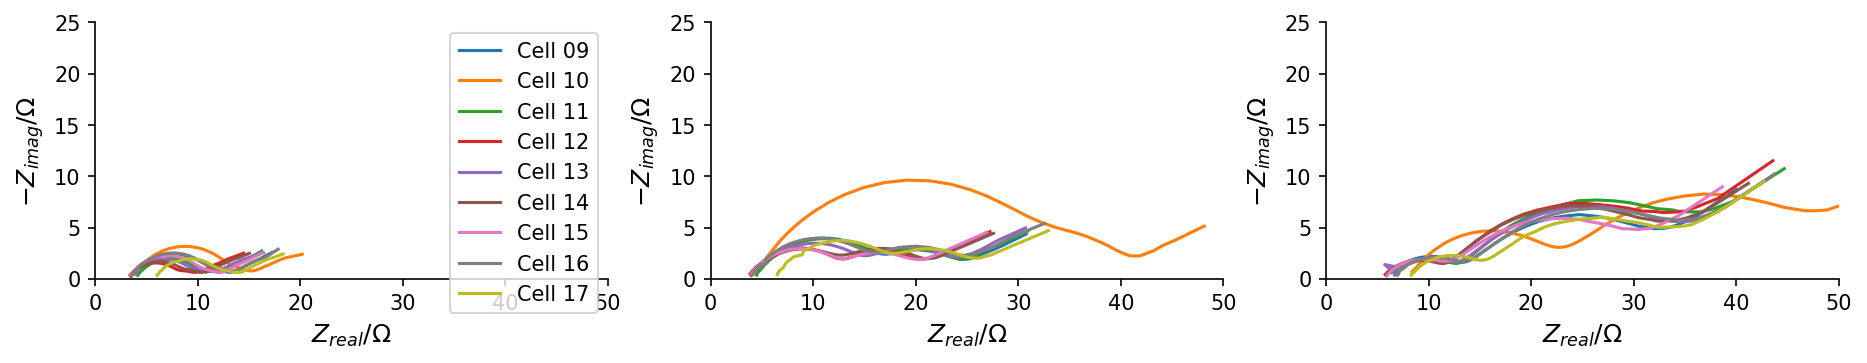
\includegraphics[width = \linewidth]{figures/results_coin/eiS_dynamic_variability.png}
  \caption{Dynamic impedance variability across nine cells at 90\%, 50\%, and 10\% state of charge during the second discharge half-cycle.
  While overall spectral features are consistent, variations in magnitude and ohmic resistance reflect manufacturing variability.}
  \label{fig:eis_dynamic_variability}
\end{widefigure}

As with any production process, cells do not respond identically but show similar behavior. One can notice impedance magnitude variations for Cell~10 and variations in the ohmic drop, which is notably higher in Cell~17 than in the others.

% Comparing complex impedance qualitatively in the complex plane across many cells in two dimensions (state of charge and state of health) is challenging. A better approach is to fit the data with a model and compare the fittedcoefficients. Not only are they fewer than the number of impedance points (10--15 versus 50), but they are also real-valued.

\subsection{Effect of the multi-sine on aging}
To assess whether continuous multi-sine excitation influences degradation, capacity retention is compared statistically in Figure \ref{fig:aging_comp}.

\begin{figure} [!h]
  \centering
  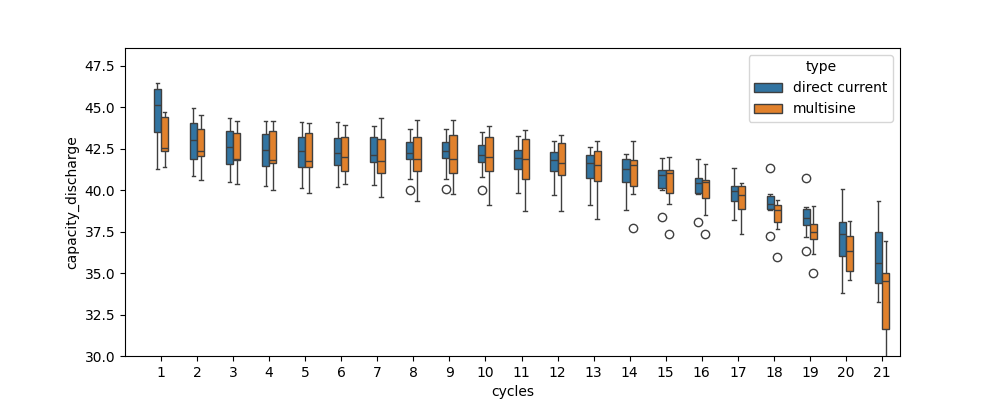
\includegraphics[width = \textwidth]{figures/results_coin/Boxplot_aging.png}
  \caption{Comparison of discharge capacity retention for cells cycled with DC-only excitation and DC with superimposed multi-sine perturbation.
  Boxplots summarize the distribution across 12 DC-only cells and 9 DEIS cells, showing no statistically significant difference under the tested conditions.}
  \label{fig:aging_comp}
\end{figure}

The reduce y-axis scale highlights the marginal differences between the two datasets, therefore I conclude that the multi-sine is not impacting the cycling performance and can be applied continously for system identification; at least for this small cells at low C-rate.

\subsection{Effect of the drift on the impedance}
Static impedance measured at different states of charge also shows good consistency. Figure~\ref{fig:eis_static_variability} reports data from three cells at the same states of charge as Figure~\ref{fig:eis_dynamic_variability}.
For reference, the variability of stationary impedance measurements obtained during interrupted cycling is shown in Figure \ref{fig:eis_static_variability}.

\begin{widefigure} [!h]
  \centering
  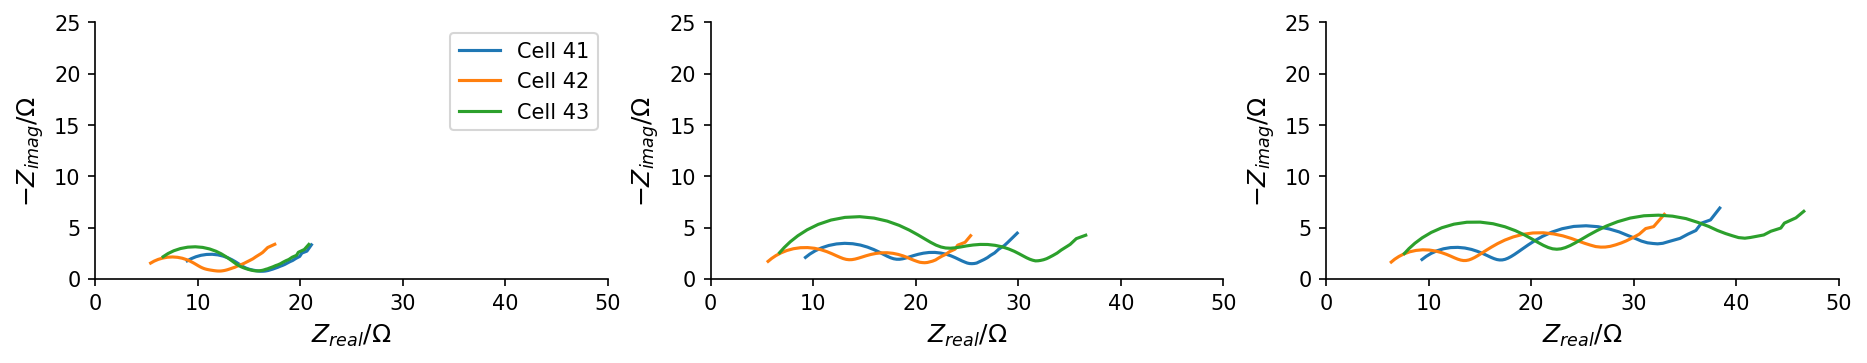
\includegraphics[width = \linewidth]{figures/results_coin/eiS_static_variability.png}
  \caption{Static impedance variability across three cells at selected states of charge.
  Impedance was measured after a 1 h rest at each state of charge using conventional stepped-sine EIS.}
  \label{fig:eis_static_variability}
\end{widefigure}

A direct comparison between static and dynamic impedance measurements is presented in Figure~\ref{fig:eis_static_vs_dynamic}.

\begin{widefigure} [!h]
  \centering
  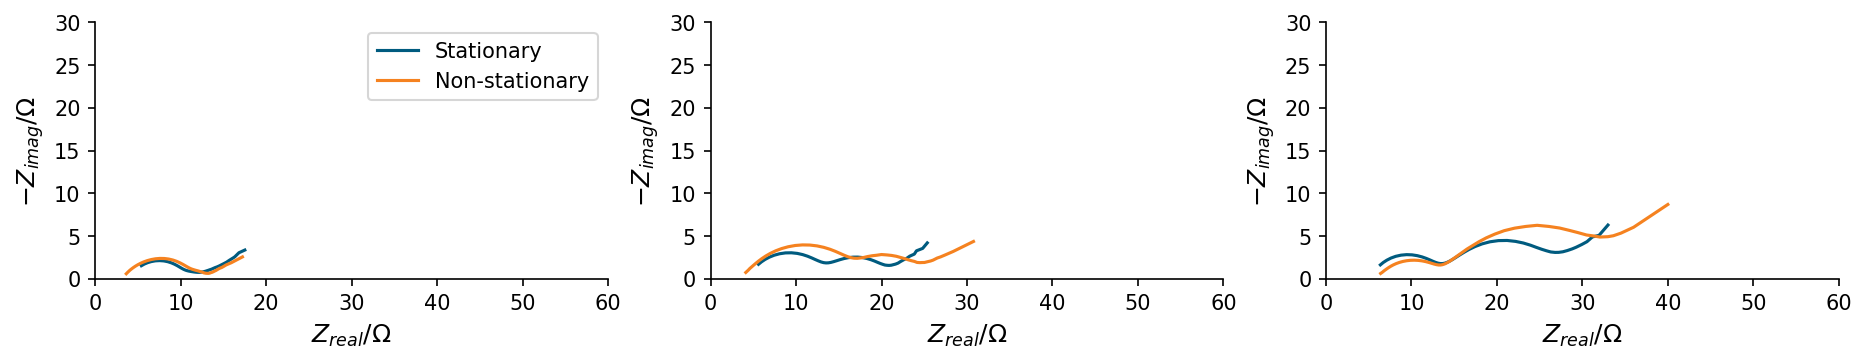
\includegraphics[width = \linewidth]{figures/results_coin/eiS_static_vs_dynamic_soc.png}
  \caption{Comparison of impedance measured under stationary conditions and during non-stationary operation at the same states of charge.
  The close agreement indicates that, at C/10, dynamic impedance measurements capture interfacial properties comparable to equilibrium EIS.}
  \label{fig:eis_static_vs_dynamic}
\end{widefigure}

This result suggests that at such a low C-rate (C/10), the electrode interfaces are in a similar state to the static case, while significantly reducing measurement time.

Comparing the classic and non-stationary measurements, it is clear how much more convenient the multisine perturbation is over the single sine, as reported in Figure \ref{fig:static vs multisine experiment}.
The latter takes around 27 hours to produce 10 spectra, while the multisine-based method outputs 270 spectra in 10 hours.

\begin{figure}[h]
  \centering
  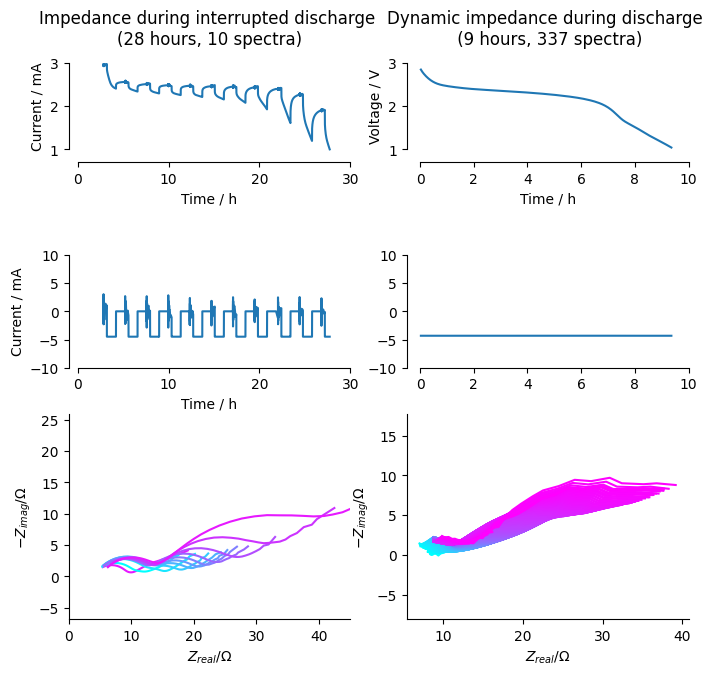
\includegraphics[width = \textwidth]{figures/results_coin/static_vs_dynamic_experiment_discharge_2d.png}
  \caption{Comparison between classic impedance measurement at different equilibrium voltages and a DEIS measurement. The classic experiments takes much longer time and produces fewer spectra. On the right hand side the multi-sine components are filtered out from voltage and current signals and only one over ten of the instantaneous impedances is plotted.}
  \label{fig:static vs multisine experiment}
\end{figure}

\section{Results of fitting}

Evaluating the fitting quality of dynamic impedance data involves multiple assessments: qualitative visualization, magnitude and structure of residuals, and consistency of model parameters across cycles.

In this work, I performed the fitting of rational polynomial functions with orders from 4 to 9. 
From the visual inspection of the fitting results, I arbitrary selected the order 5 because it can represent all the different shapes of instantaneous impedance, as shown in Figure~\ref{fig:results_fitting_coin_cycle5} with the minimum number of parameters. 
The residuals are small for the real part, approximately 1\%, but larger for the imaginary part. The systematic structure of the residuals, especially the pronounced deviations at the highest three frequencies, indicates that the model does not fully reproduce all spectral features of the dataset. 
I believe, this issue is both related to the arbitrary choice of the weighting factors in the least-square objective function and the solver itself.

\begin{figure}[!b]
  \centering
  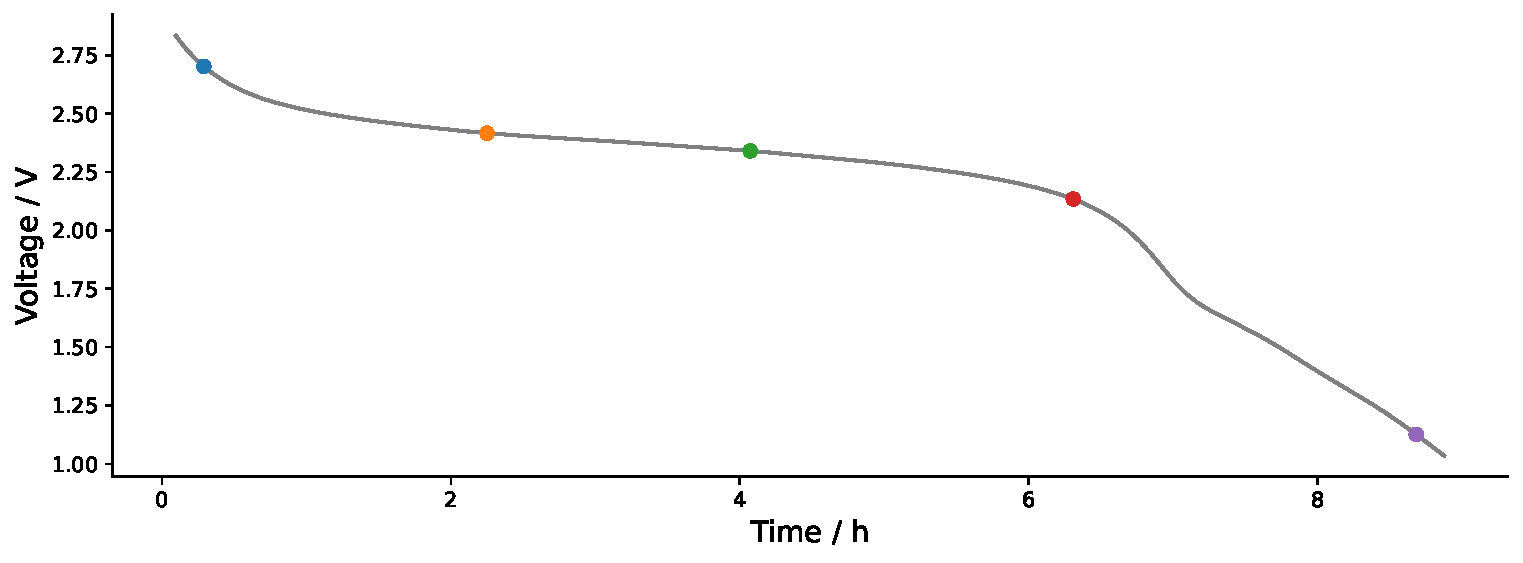
\includegraphics[width=\textwidth]{figures/results_coin/fit_cell009_order5_cycle_5_sequence_4_index_[7, 78, 144, 225, 311].pdf}
  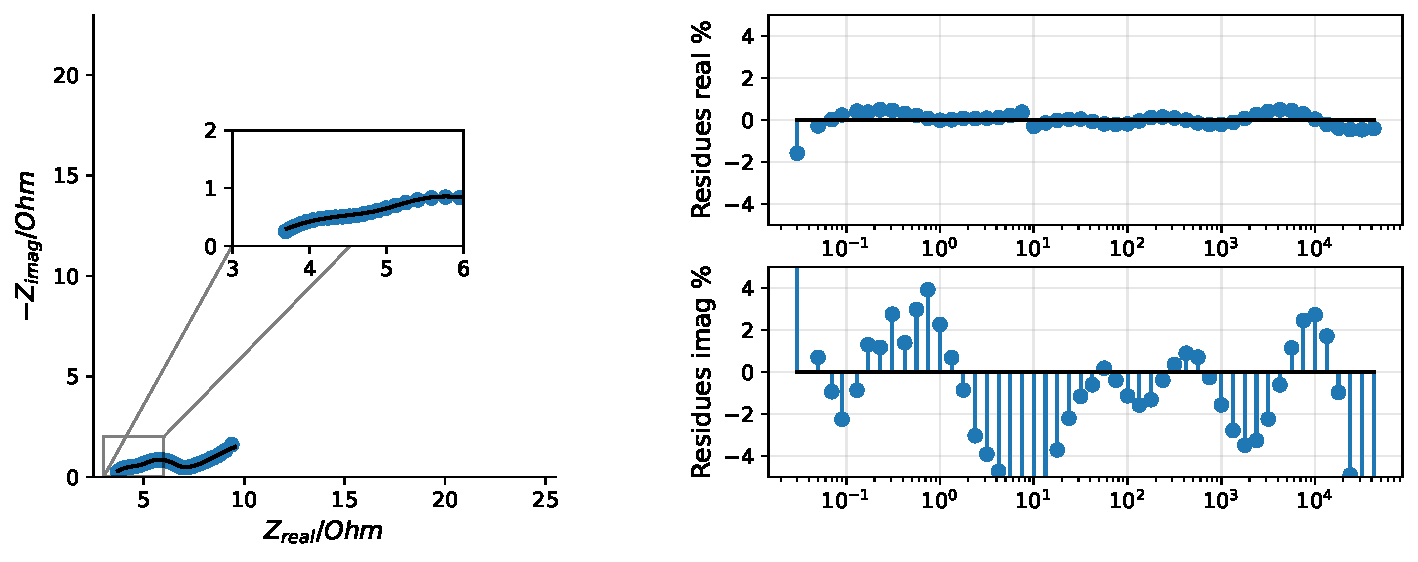
\includegraphics[width=\textwidth]{figures/results_coin/fit_cell009_order5_cycle_5_sequence_4_index_7.pdf}
  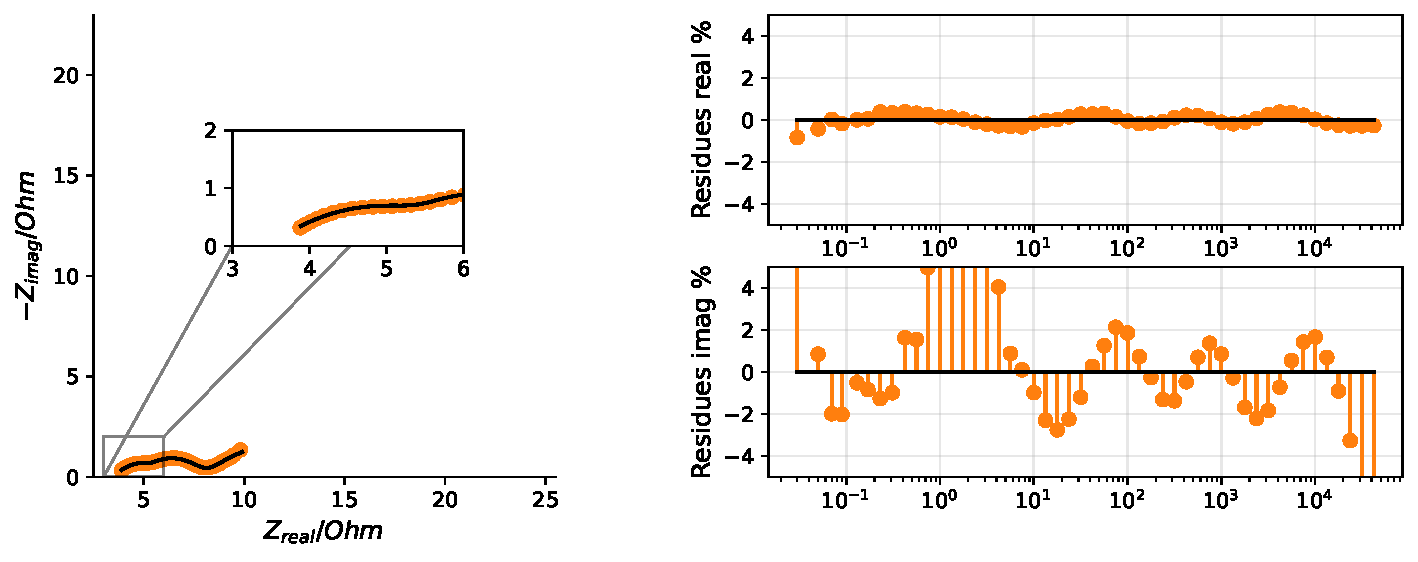
\includegraphics[width=\textwidth]{figures/results_coin/fit_cell009_order5_cycle_5_sequence_4_index_78.pdf}
  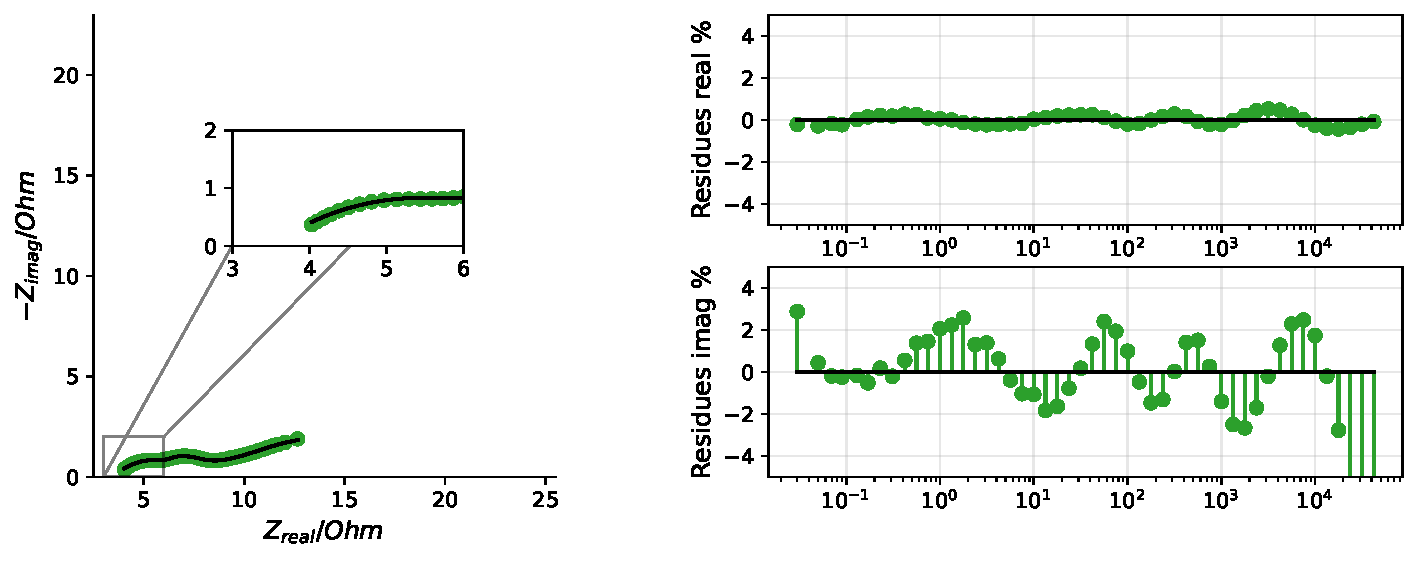
\includegraphics[width=\textwidth]{figures/results_coin/fit_cell009_order5_cycle_5_sequence_4_index_144.pdf}
  \caption{Rational polynomial fitting of dynamic impedance spectra at different states of charge (marked with colors dots) during discharge of cycle 6.
  The figures in the panel after the voltage time series report the impedance data (markers) and fit result (solid black line). Residuals are reported next to each spectrum. The colors of the markers represents the states of charge.}
  \label{fig:results_fitting_coin_cycle5}
\end{figure}
% \clearpage
\begin{figure}[!ht]\ContinuedFloat
  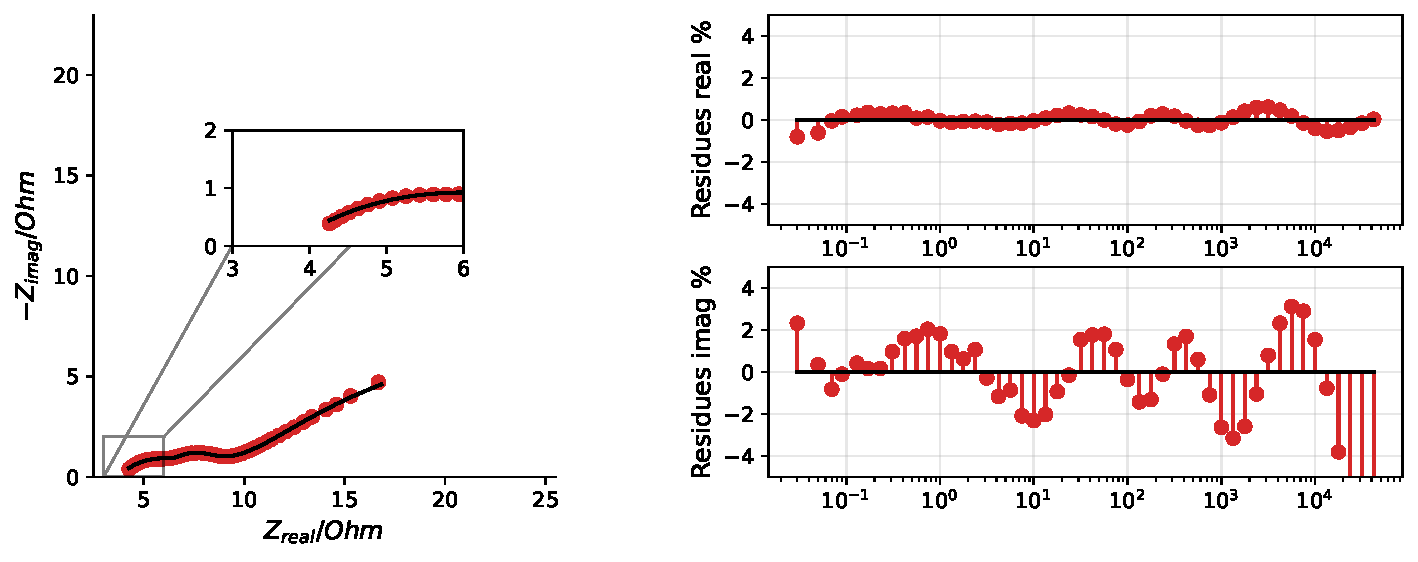
\includegraphics[width=\textwidth]{figures/results_coin/fit_cell009_order5_cycle_5_sequence_4_index_225.pdf}
  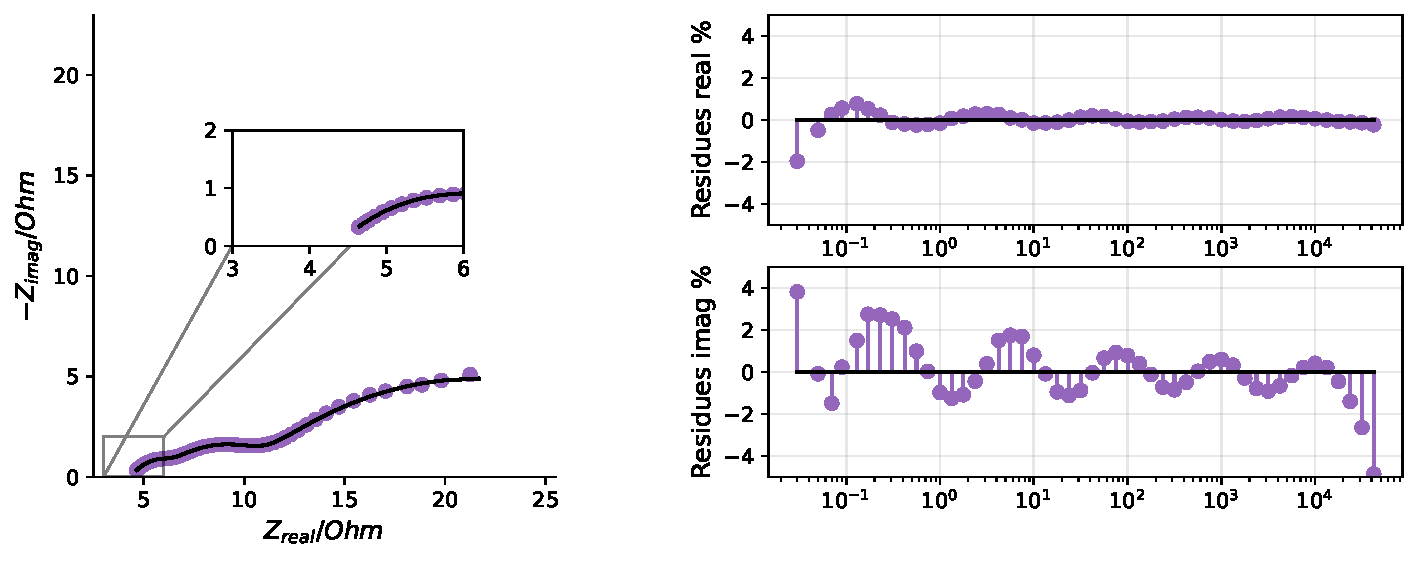
\includegraphics[width=\textwidth]{figures/results_coin/fit_cell009_order5_cycle_5_sequence_4_index_311.pdf}
  \caption[]{Continued}
  % \caption{Rational polynomial fitting of dynamic impedance spectra at different states of charge during discharge of cycle 6.
  % Symbols represent measured impedance; solid lines show the fitted model.
  % Residuals are reported below each spectrum.}
\end{figure}

Despite the small residual magnitudes, their oscillatory behavior persists for polynomial orders up to nine (the highest tested). 
In a well-posed regression problem, residuals are expected to be randomly distributed with magnitude comparable to the measurement variance. 
The persistence of structured oscillations therefore indicates that the limitation is not simply insufficient model order.
The fitting with a smaller order of 4, doesn't lead to a correct representation of the impedance since the model is not capable of resolve the two semicircles at higher frequency. This issue could not be connect with the model structure, but rather the arbitrary weighting factor used in the regression problem.

Despite the criticalities it is interesting to look at the fitting result for order 5 to have an idea of the advantage of parameterization. The fitted parameters vary smoothly across state of charge and state of health although some abrupt magnitude changes are observed when the impedance manifests a new feature (or the features disappears) and the model must adapt to it. 
Representing complex-valued impedance through real-valued model parameters provides a compact description of the spectrum and facilitates subsequent data-driven modeling of cell aging. 
The fitted coefficients can therefore be used as features for machine-learning models to predict state of health.

The evolution of the fitted parameters during cycle~2 across all electrochemical techniques is illustrated in Figure~\ref{fig:fitting_parameters_cycle2}. 
Parameters $a_1$ (orange line) and $a_3$ (red line) exhibit abrupt transitions when a new spectral feature becomes significant: a semicircle emerges at high state of charge and gradually merges into another high-frequency semicircle. 
The parameter jump occurs because the regularized least-squares procedure allow the parameters to increase only when the residual contribution in that region becomes sufficiently large to significantly impact the cost function. 

\begin{figure}[!h]
  \centering
  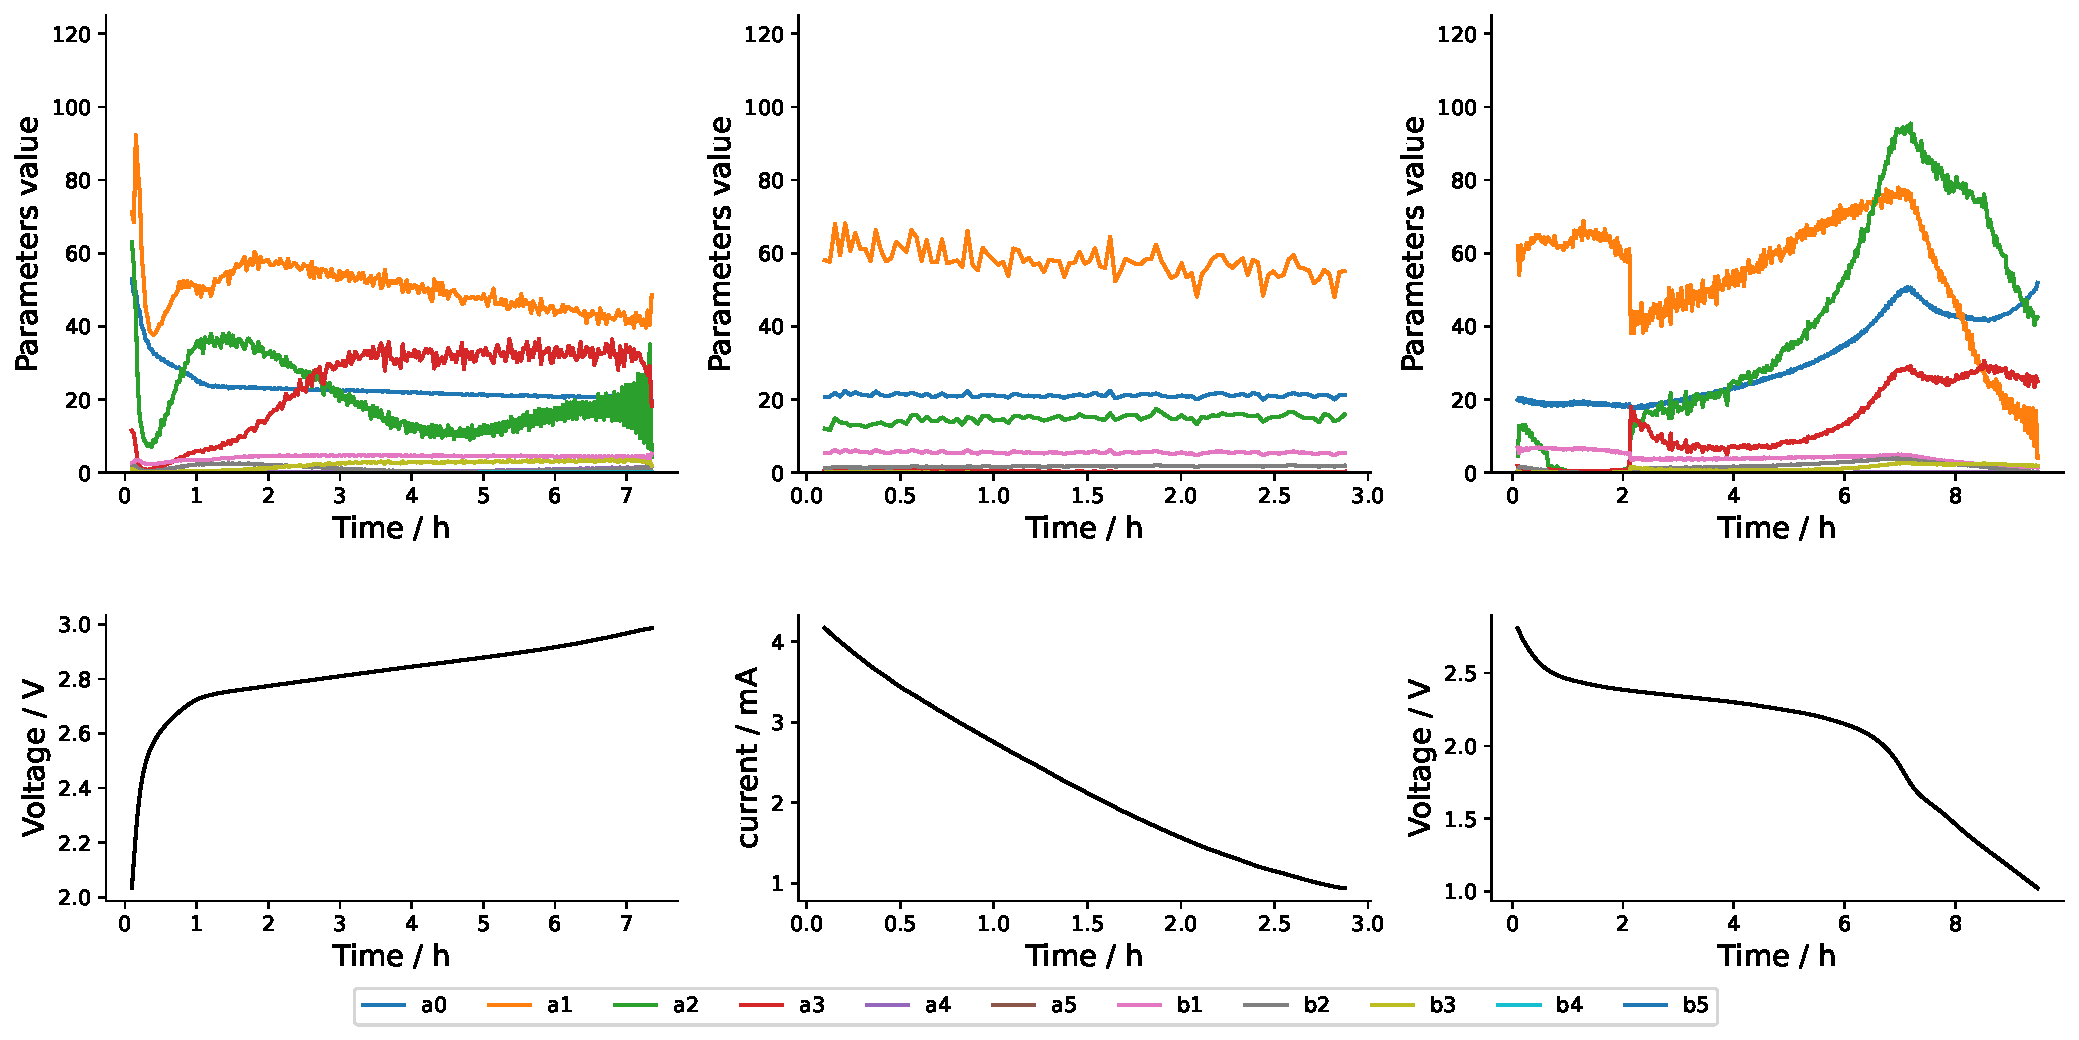
\includegraphics[width = \textwidth]{figures/results_coin/Cell009_fitting_parameters_ouput_order5_cycle1.pdf}
  \caption{Upper row: fitted rational polynomial parameters for all techniques during cycle 2.
  Lower row: corresponding cell voltage and current reconstructed via DMFA.
  Abrupt parameter changes correspond to the emergence of new impedance features.}
  \label{fig:fitting_parameters_cycle2}
\end{figure}

As shown in Figures~\ref{fig:deis_aging_charge} and~\ref{fig:deis_aging_discharge}, after cycle~5 the impedance shape stabilizes, showing two consecutive semicircles followed by a diffusive feature. 
This stabilization is reflected in the corresponding fitted parameters for cycle~5 (Figure~\ref{fig:fitting_parameters_cycle5}) and subsequent cycles (e.g., cycles~10, 15, 20, and 22). 
Parameter magnitudes and trends are largely preserved across cycles and remain mostly continuous within the techniques of the same cycle. 
These observations suggest that, despite their numerical limitations, the fitted parameters capture systematic changes correlated with state of charge and state of health. 
The same qualitative behavior is observed in the results of the other cells.

\begin{figure}[!h]
  \centering
  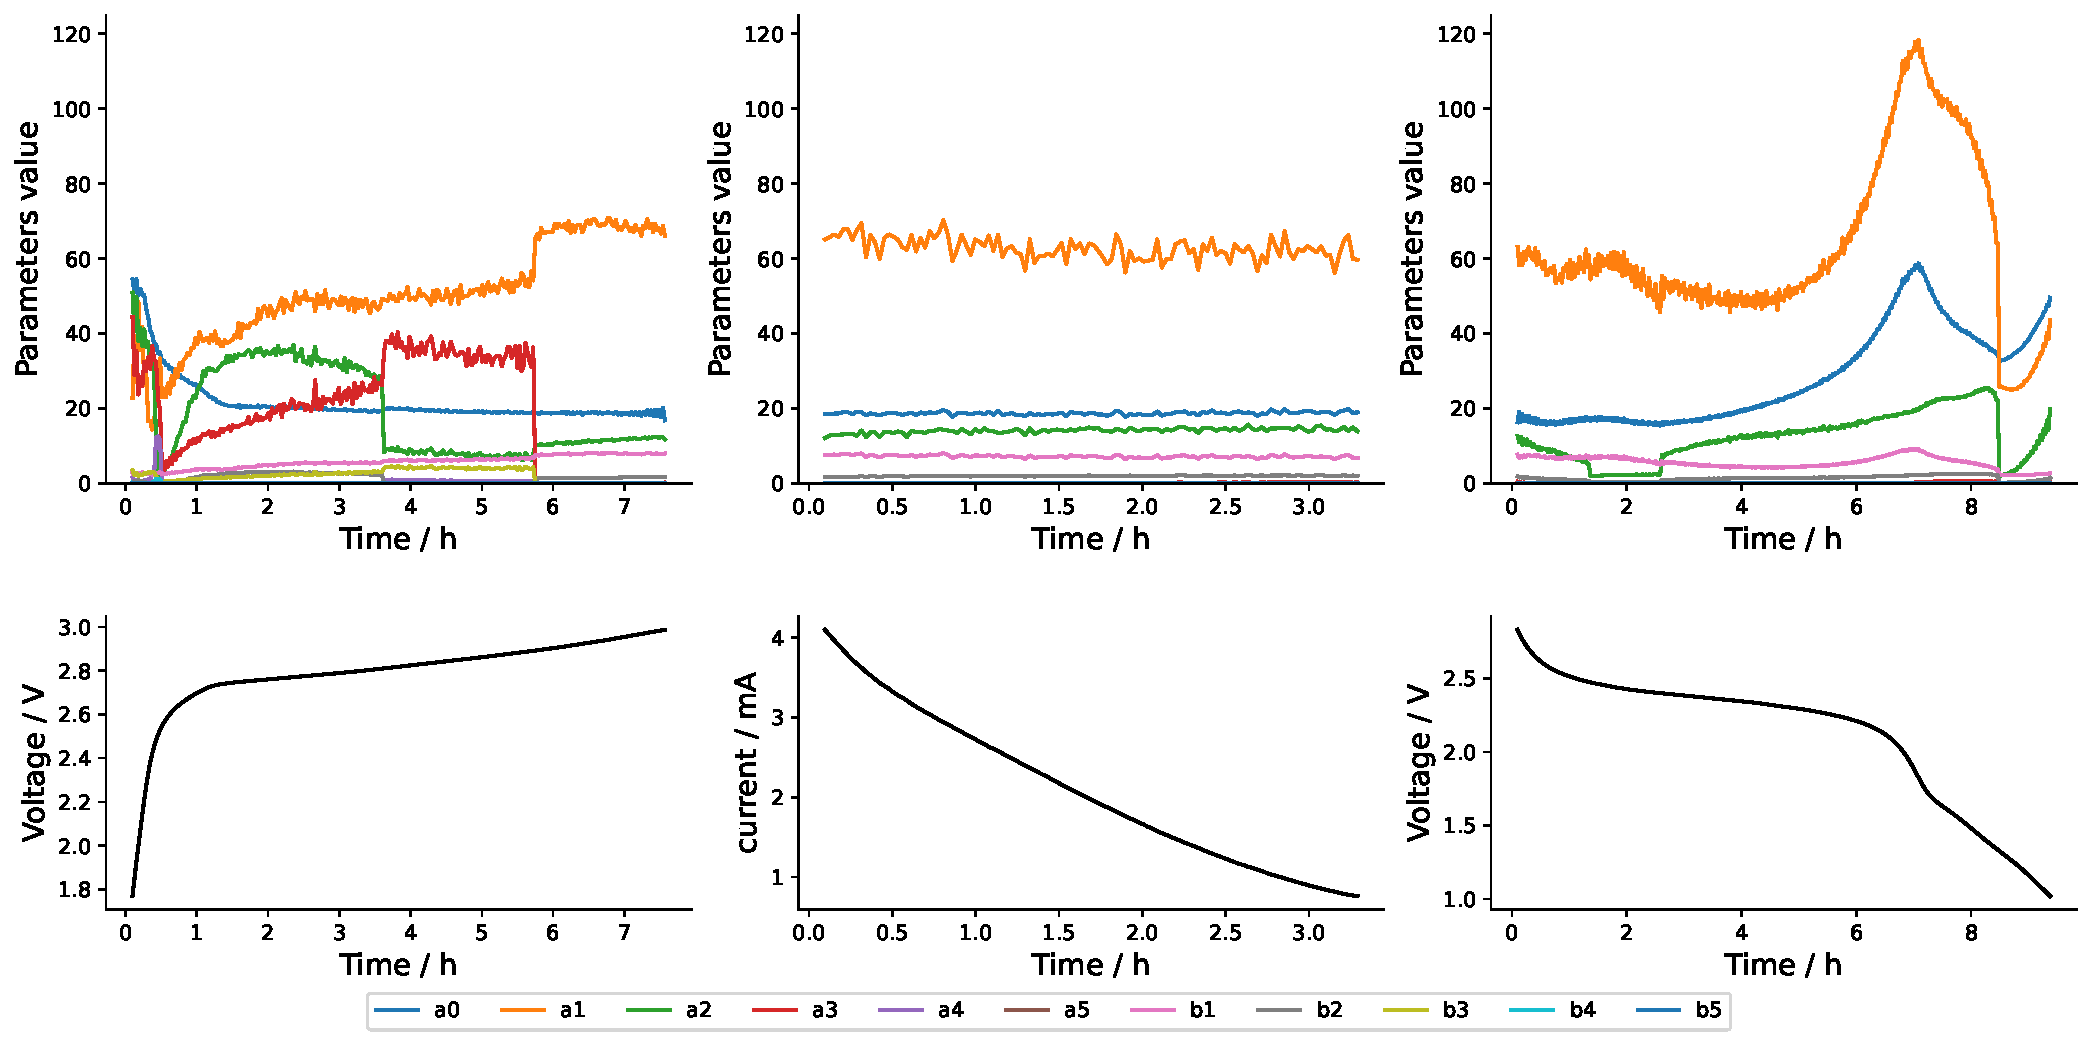
\includegraphics[width = \textwidth]{figures/results_coin/Cell009_fitting_parameters_ouput_order5_cycle4.pdf}
  \caption{Upper row: fitted rational polynomial parameters for all techniques during cycle 5.
  Lower row: corresponding cell voltage and current reconstructed via DMFA.}
  \label{fig:fitting_parameters_cycle5}
\end{figure}

\begin{figure}[!h]
  \centering
  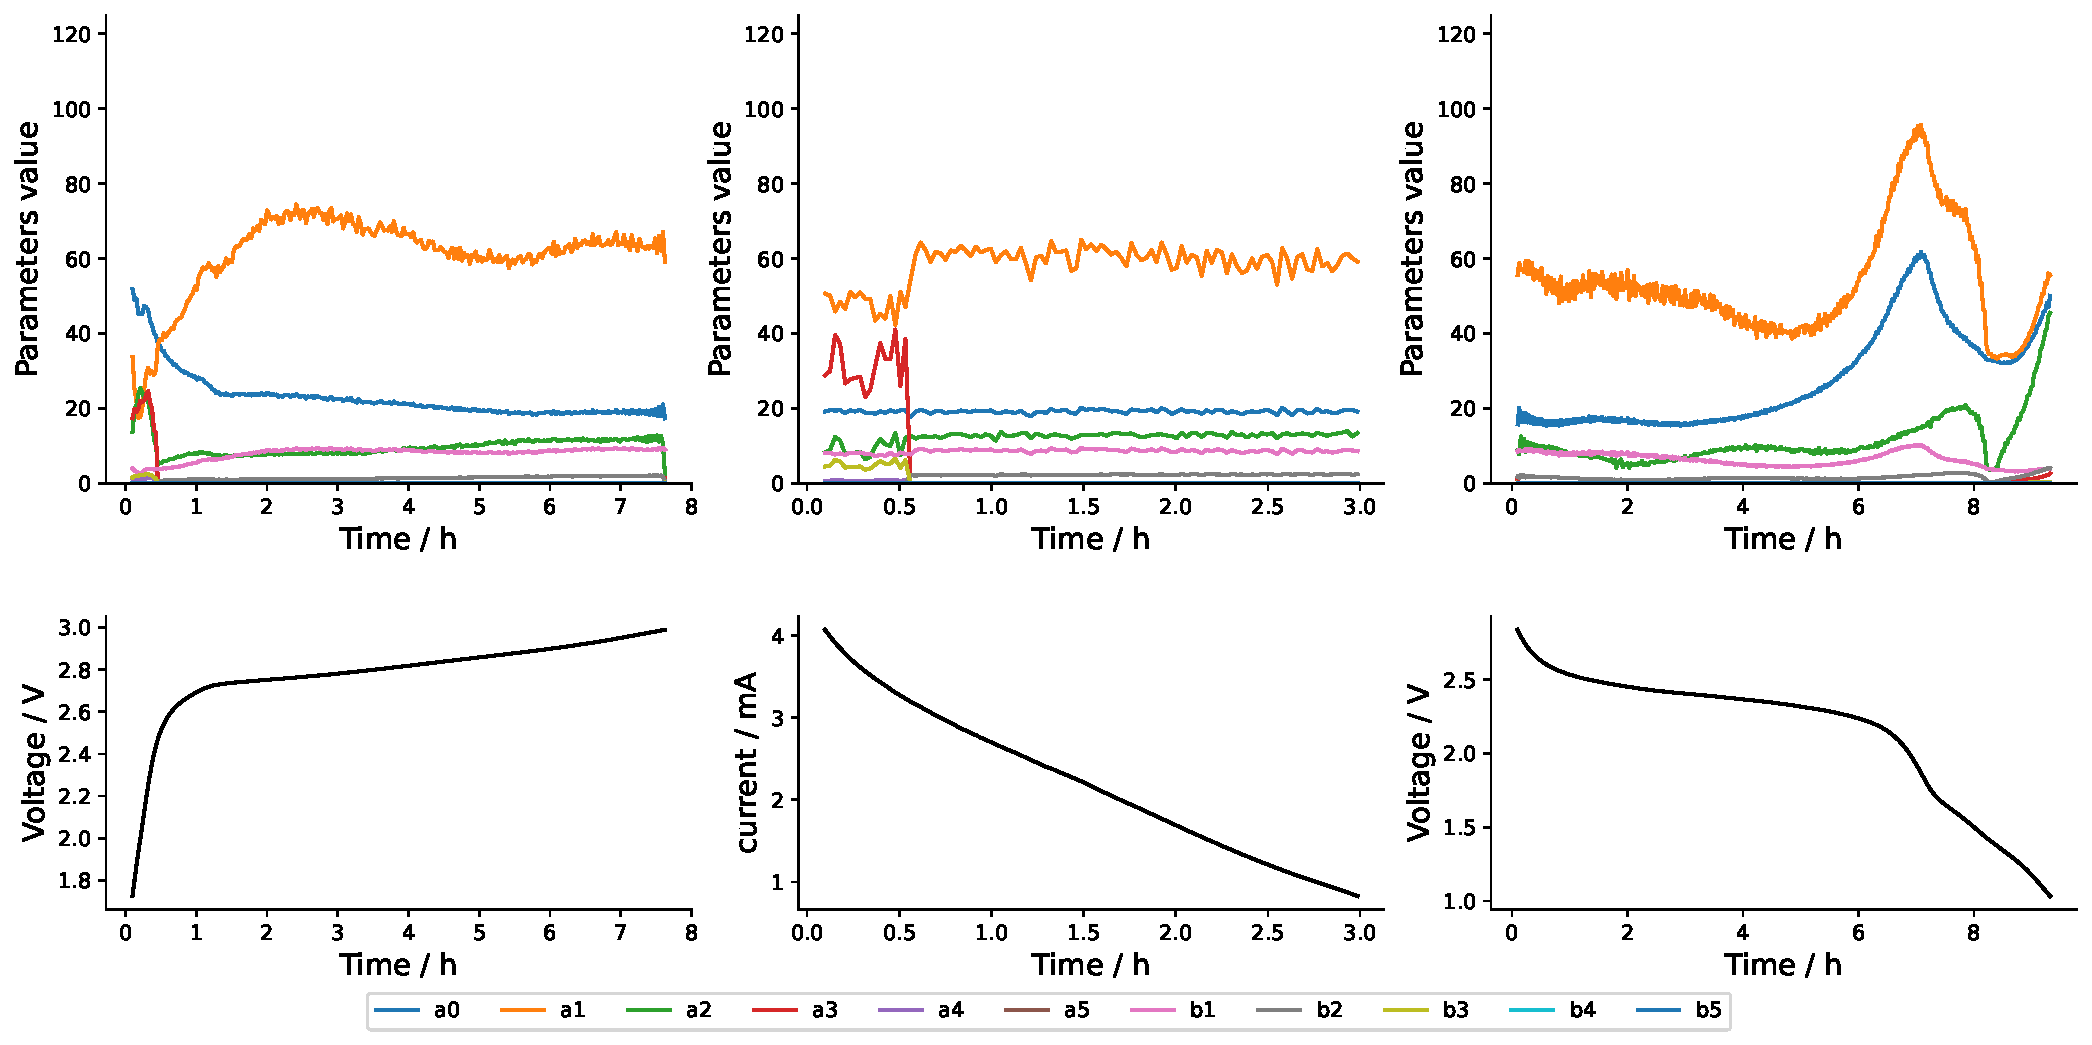
\includegraphics[width = \textwidth]{figures/results_coin/Cell009_fitting_parameters_ouput_order5_cycle9.pdf}
  \caption{Upper row: fitted rational polynomial parameters for all techniques during cycle 10.
  Lower row: corresponding cell voltage and current reconstructed via DMFA.}
  \label{fig:fitting_parameters_cycle10}
\end{figure}
\clearpage
\begin{figure}[!h]
  \centering
  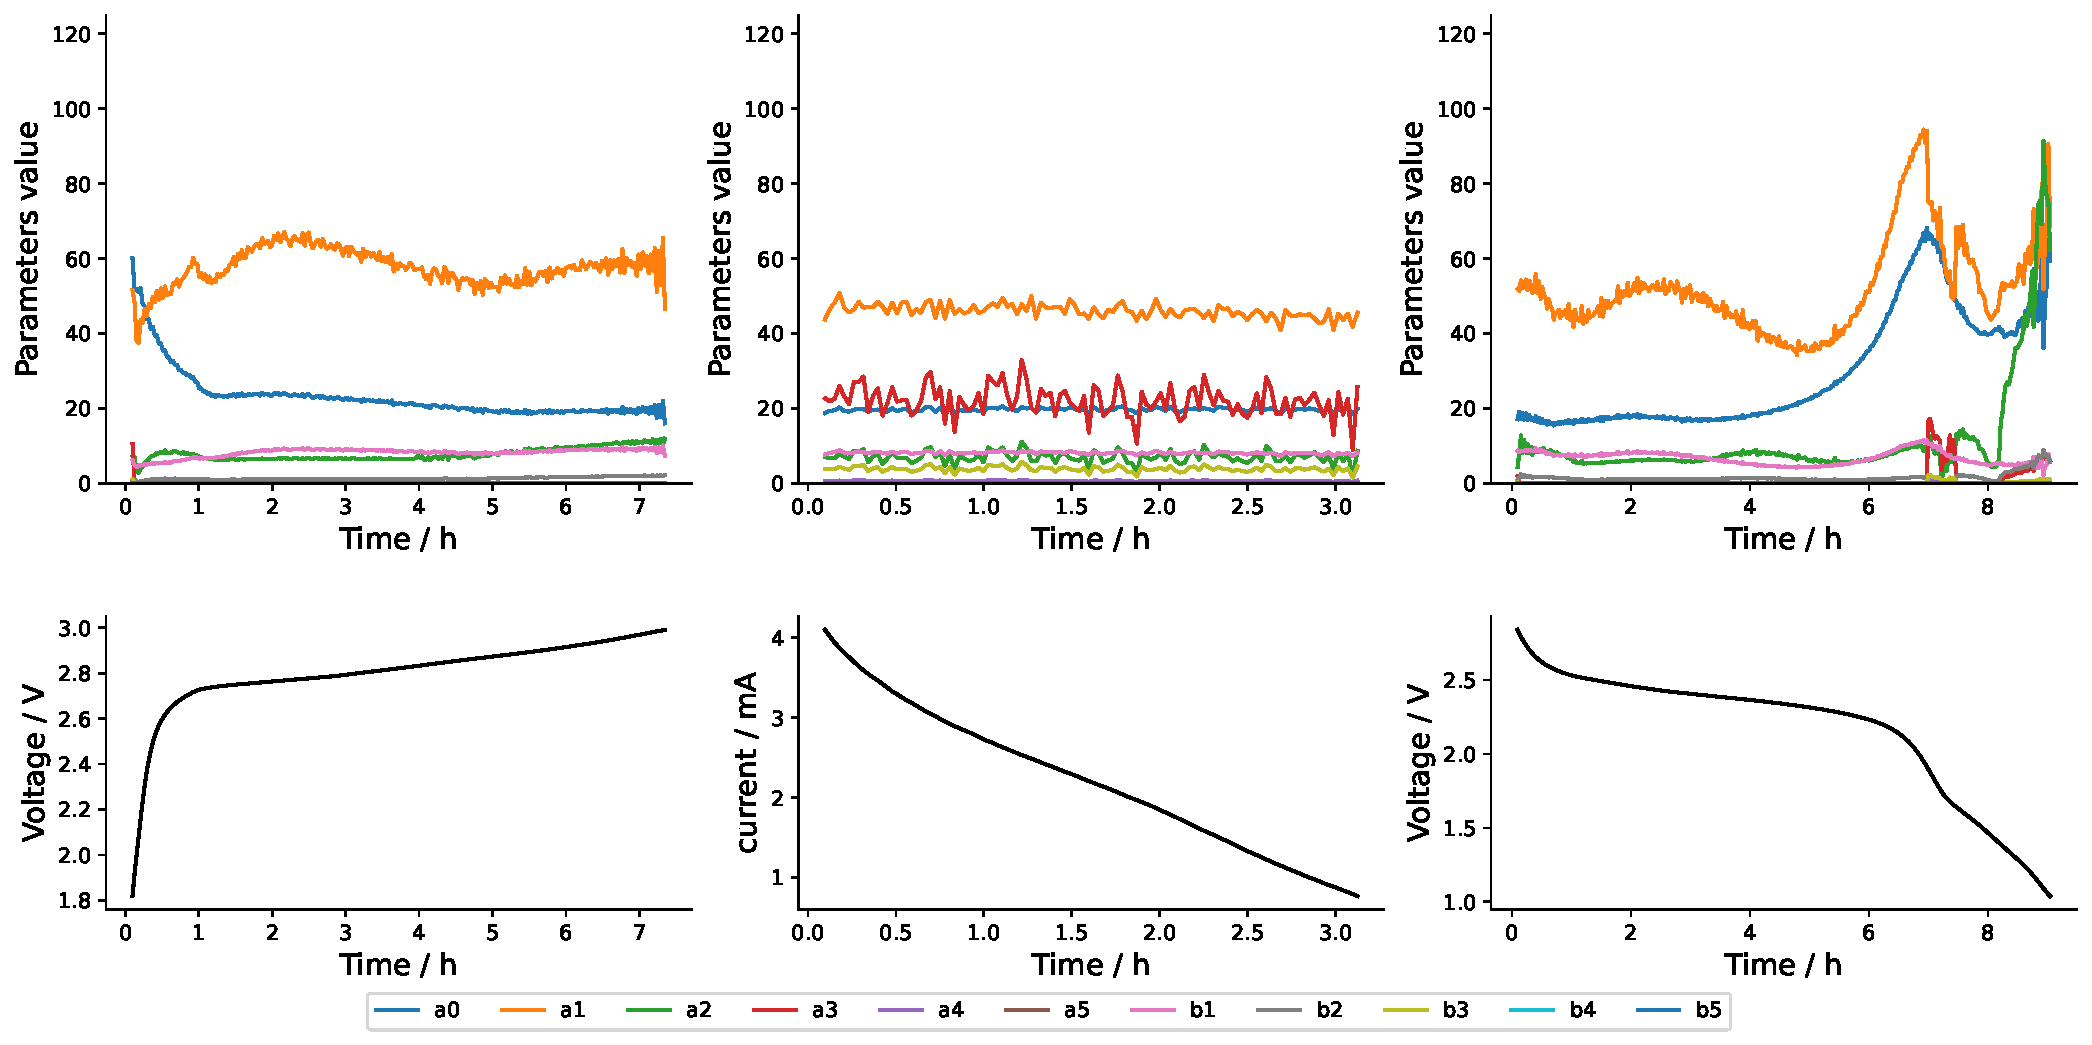
\includegraphics[width = \textwidth]{figures/results_coin/Cell009_fitting_parameters_ouput_order5_cycle14.pdf}
  \caption{Upper row: fitted rational polynomial parameters for all techniques during cycle 15.
  Lower row: corresponding cell voltage and current reconstructed via DMFA.}
  \label{fig:fitting_parameters_cycle15}
\end{figure}
\begin{figure}[!h]
  \centering
  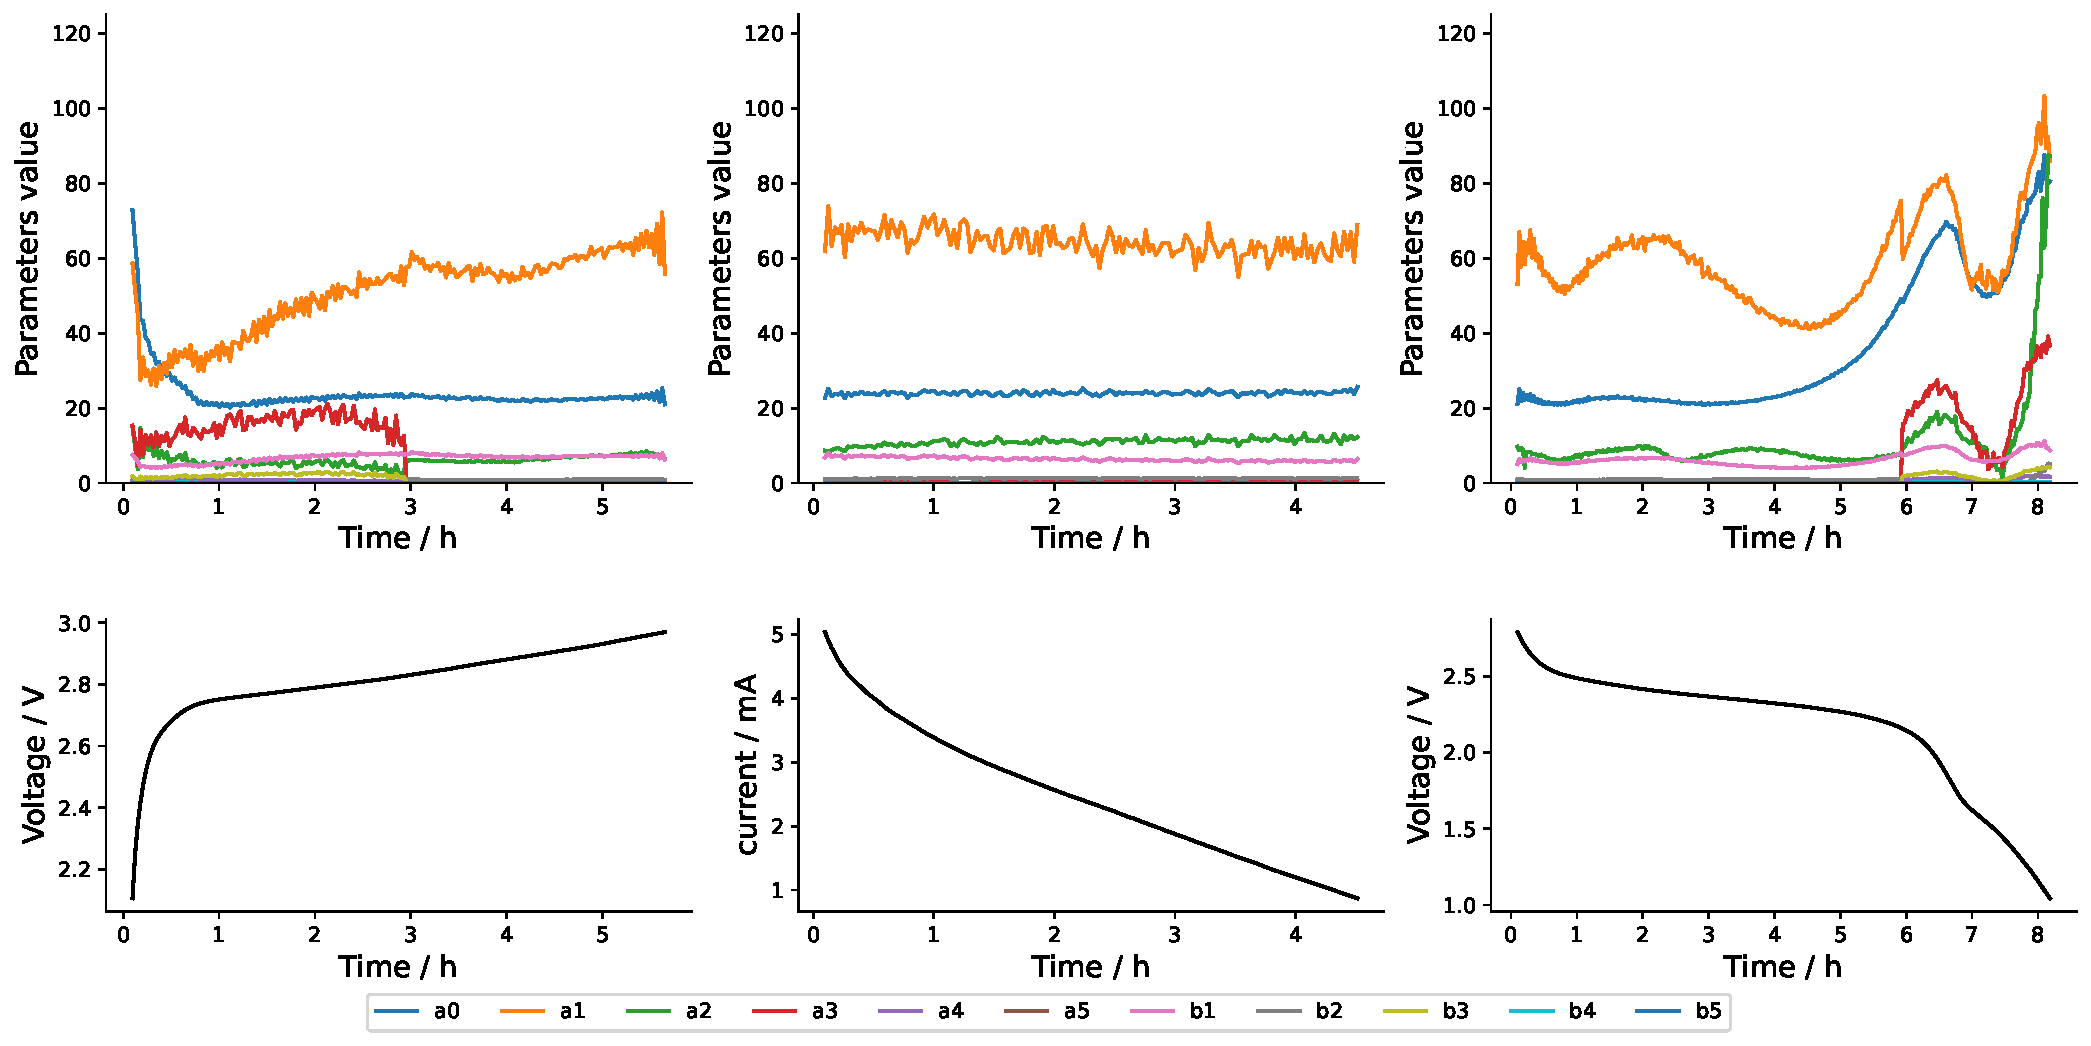
\includegraphics[width = \textwidth]{figures/results_coin/Cell009_fitting_parameters_ouput_order5_cycle19.pdf}
  \caption{Upper row: fitted rational polynomial parameters for all techniques during cycle 20.
  Lower row: corresponding cell voltage and current reconstructed via DMFA.}
  \label{fig:fitting_parameters_cycle20}
\end{figure}
\begin{figure}[!h]
  \centering
  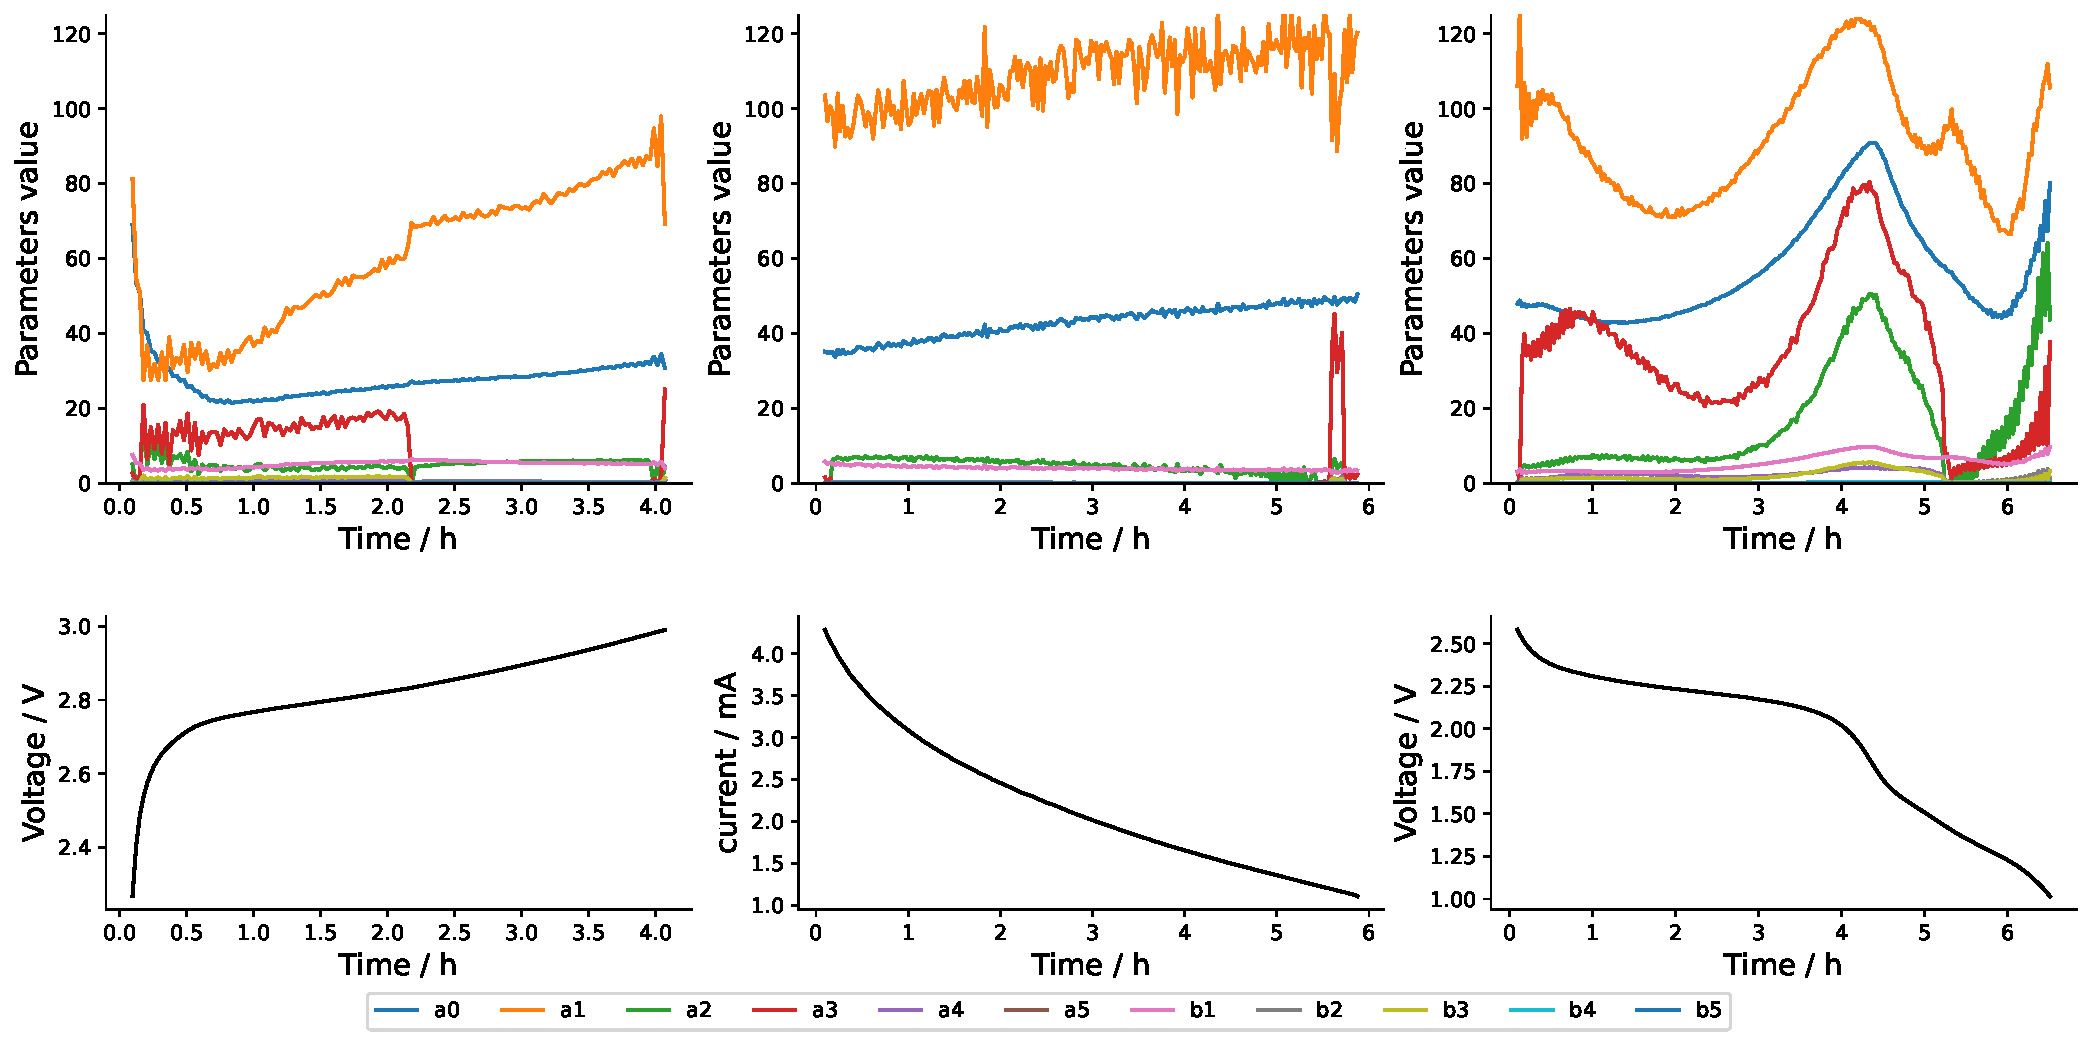
\includegraphics[width = \textwidth]{figures/results_coin/Cell009_fitting_parameters_ouput_order5_cycle21.pdf}
  \caption{Upper row: fitted rational polynomial parameters for all techniques during cycle 22.
  Lower row: corresponding cell voltage and current reconstructed via DMFA.}
  \label{fig:fitting_parameters_cycle22}
\end{figure}

However, the persistence of oscillatory residuals with increasing polynomial order, together with the systematic disparity between numerator and denominator coefficient magnitudes, reveals a structural limitation of the adopted identification formulation. 
In the least-squares estimation of rational polynomial transfer functions, the problem is \emph{ill-posed} in the sense of inverse problem theory: small perturbations in the measured impedance (e.g., noise or minor spectral features) can produce disproportionately large variations in the estimated parameters, and multiple distinct parameter sets may generate nearly indistinguishable impedance responses \cite{vogelComputationalMethodsInverse2002, ljungSystemIdentificationTheory1999}. 

This behavior is reflected in the observation that denominator coefficients often assume very small magnitudes while numerator coefficients span a significantly larger dynamic range. 
Such scaling imbalance indicates that the optimizer compensates local spectral mismatches primarily through numerator adjustments while maintaining a weakly constrained denominator structure. 
Mathematically, this corresponds to a poorly conditioned Jacobian matrix and strong correlation among parameters. 
Under these conditions, increasing the number of coefficients does not necessarily improve robustness; instead, it can lead to near pole-zero cancellations, ill-scaled parameters, and structured residuals that are not consistent with purely stochastic measurement error.
The impedance spectrum can often be reproduced accurately in magnitude, but the corresponding parameter values may not be uniquely determined or numerically stable. 
This explains why increasing model order beyond five does not eliminate oscillatory residuals and does not significantly improve parameter consistency.

Over the past three decades, alternative identification frameworks have been developed in system identification, control engineering, and RF network modeling to address precisely these issues. 
Methods such as vector fitting estimate poles and residues of rational approximations in a structured and numerically stable manner, allowing automatic determination of effective model order and reducing sensitivity to noise \cite{gustavsenRationalApproximationFrequency1999,gustavsenImprovingPoleRelocating2006}. 
Similarly, realization-based approaches such as the Loewner framework construct minimal state-space representations directly from sampled frequency data using singular value decomposition, with the model order inferred from the spectral content rather than prescribed a priori \cite{antoulasApproximationLargeScaleDynamical2005, mayoFrameworkSolutionGeneralized2007}. 
These methods do not require manual smoothing parameters and generally produce more stable dynamical representations of the impedance response, but the knowledge of industrial mathematics limits the applicability in the chemical and engineering community.
Nevertheless, the rational polynomial parametrization adopted here remains useful as a compact descriptive tool and as an initial framework for transforming complex impedance spectra into real-valued feature trajectories.

\section{Summary and implications}

In this chapter, dynamic electrochemical impedance spectroscopy was applied to commercial lithium-based coin cells operated under non-stationary charge/discharge cycling using a typical constant current--constant voltage protocol.
The objective was not to extract detailed physicochemical parameters, but to validate the proposed DEIS methodology at the full-cell level and assess its consistency, robustness, and impact on battery operation.

Continuous impedance spectra were successfully acquired throughout cycling using a broadband (7 decades) multi-sine excitation combined with online and offline signal processing.
The resulting dynamic impedance measurements capture the evolution of interfacial resistance, charge-transfer processes, and diffusion-related features as functions of both state of charge and state of health.
Comparison with classical stationary EIS measurements performed during interrupted cycling shows good agreement within the experimental variability of the cells, indicating that at moderate C-rates (C/10), the non-stationary operating conditions do not significantly alter the electrochemical state of the interfaces.

Importantly, statistical comparison of capacity retention demonstrates that continuous superimposition of the multi-sine perturbation does not affect cell aging under the investigated conditions.
This result supports the practical applicability of DEIS for long-term experiments without compromising cell integrity, at least for small-format cells and low to moderate current densities.

Dynamic impedance spectra were fitted using rational polynomial models through complex nonlinear least-squares with regularization.
Although the chosen black-box model does not provide direct physical interpretation of individual electrochemical processes, it enables real-valued parametrization of impedance evolution across cycles.
The smooth variation of fitted parameters with state of charge and state of health suggests that such representations may serve as effective features for data-driven aging diagnostics.

At the same time, the limitations of full-cell impedance analysis are evident.
The superposition of positive and negative electrode responses leads to complex models that may not be fully represented by a rational polynomial, as evidenced by oscillatory residuals.
Furthermore, a single model has limited ability to represent impedance across all operating conditions.

Nevertheless, the flexibility of rational polynomials is promising.
With proper characterization of the actual measurement error structure and systematic exploration of regularization penalty factors, the robustness of the fitting can be improved.
I suggest conducting a study with simulated electrochemical impedance data where the degrees of freedom and noise levels are known a priori.
\input{chapters/10_silicon_carbonitrate}
\input{chapters/11_lithium_sodium_iron_phosophate}
\input{chapters/12_capacitors}
\chapter{Conclusions}

\section{Summary of contributions}
% Intro with summary
This work presents a complete methodology for the acquisition of impedance spectra in non-stationary electrochemical systems. The novelty reported here is the use of automation and online computation to measure impedance in a wide band of frequency continuously during the cycling of batteries.

Before this work, the impedance of batteries in non-stationary conditions had been measured only for short times and limited frequency bands. That misses the characterization of the entire frequency response of batteries or its degradation. The main cause is the technical difficulty of managing and storing high sampling frequency signals and the estimation of the instantaneous impedance from them.

Continuous sampling at 250 kSa/s would generate ~4.3 GB per hour per channel, making multi-week battery studies impractical. Previous dynamic impedance work was therefore limited to short experiments (minutes to hours) or narrow frequency bands that could be sampled at lower rates.

I solved this problem by extending an existing hardware configuration (commercial potentiostat, waveform generator, and oscilloscope) with custom automation software that synchronizes the devices, manages data streaming, and performs online impedance calculation for high frequencies before data storage. The impedance of the low frequencies is calculated offline after the experiment with existing methods.

The complete software stack is released as open-source Python libraries:
\begin{itemize}
\item Multisine: Excitation signal generation and optimization; 
\item pyeclab, pypicostreaming, TrueFormAWG: Remote control of set-up components;
\item DEIStools: Multi-channel automation, online processing, impedance calculation lagorithms and data visualization.
\end{itemize}
This effort reduces the technical barrier (using commercial instruments) to perform long-term dynamic ipedance experiments and allows more scientist to get into the topic.

The modular nature of the software library permits to adapt the method for devices of other brands or modify the online processing calculation whihle keeping the core logic of the automation untouched.

I demonstrated the applicability of the method for commercial coin cell batteries made of manganese oxide and lithium/aluminum alloy acquiring the instantaneous impedance throughout their cycling lifetime. A multi-sine excitation is continuously applied and the spectra are computed with a time resolution of 100s. The impedance, estimated in the broadband frequency of 10mHz to 100kHz shows correlation with the state of charge and state of health. The measurement shows reproducibility over 9 cells and the analysis shows no alteration of the aging caused by the multi-sine excitation when compared to the control experiment set.

The instantaneous impedance estimated via multi-sine excitation in non-stationary condition removes any overhead time usually present for stationary impedance during interrupted cycling and reduces the time for the estimation of a single spectrum bringing not only a saving of time but also 25 to 30 times more spectra. With around 1000 spectra per cell across 30 cycles at a C-rate of C/10, dynamic impedance is a promising source of data for data-driven modeling approaches of batteries. While physical modeling for batteries is complicated and prone to overparametrization, a simpler black-box model could be a valid alternative for practical and cell-specific implementation.

This initial validation step is very promising and I suggest further investigation using bigger format cells and standard electrode materials such as lithium nickel cobalt manganese oxide, lithium iron poshpate and graphite.

The C/10 rate used in this validation study represents a conservative starting point where drift is slow relative to perturbation frequencies. Extension to higher C-rates (1C and above) will require careful consideration of the time-frequency resolution trade-off and validation that the system remains quasi-stationary on the timescale of the multisine period.

% Other measurements
Dynamic impedance spectroscopy is not restricted to full cell applications. In this work I also included experiments for the electrochemical characterization of single electrodes for Faradaic and non-Faradaic energy storage types in three-electrode laboratory cells. In this case, the separation of the electrodes impedance by the presence of a reference electrode makes the physical interpretation easier and enabled extraction of kinetics parameters using existing physical models.

The first case-study was lithium titanium phosphate for sodium ion intercalation as possible active material in aqueous sodium-ion battery negative electrodes. Here we showed the difference in the impedance obtained when the drift is a constant current, typical for battery characterization, or cyclic voltage sweep, typical in electroanalytics. The instantaneous impedance of the working electrode shows how the surface kinetics is slowed down when the peak of the voltammetry is approached and suggests why intercalation materials should be studied with the constant current technique. 

We fitted a physical model for ion intercalation with porous electrode theory to the data of one charge and discharge cycle with galvanostatic drift to estimate the kinetics parameters. The most interesting finding was the asymmetry in the charge transfer process between charge and discharge that we interpreted as a difference in solvation and desolvation activation energy. 

The other case-study was an electrical double layer capacitor made of symmetric activated porous carbon electrodes in an aqueous solution of KF in a three-electrode Swagelok type cell. Here, we experimented with the instrumental set-up using two channels of a potentiostat with one scope each for the acquisition of full cell and half cell voltages that allows for the separated estimation of the impedance for positive and negative electrode. Such experiment demonstrates that even in symmetric systems the impedance of the electrodes is different because of the history and electric potential. This type of experiment can also identify cross-talk between the electrodes while the electrochemical device is cycling. In fact, the second channel of the workstation is used only to measure the voltage drop of one half-cell (the other is deduced by subtraction with the full-cell voltage).

Another interesting result is about the position of the reference electrode. On the same cell, we positioned the tip of the reference electrode outside the electrodes stack and then in the middle of it, between two separators, obtaining the appearance of an artifact in the impedance in the first case as obtained in some theoretical investigation.

We used again a physical model for the adsorption of ions on porous electrodes to estimate the kinetics parameters from the impedance data, although it doesn't change significantly during the cycling.

In these two experiments we focused only on the impedance change within a cycle since at that time the instrumental set-up was not yet automatized. I suggest a follow-up project in which the impedance of single interfaces in three-electrode cells is measured over multiple cycles to characterize the degradation.

% Preliminary measurements
I also conducted explorative measurements on anodes for lithium- and sodium-ion batteries in compact systems with organic electrolytes. The goal was of characterize the storage mechanisms and identifying side reactions, mainly ion electrodeposition. After some tests on Swagelok type cells I realized the best cell geometry for this experiment is the pouch cell with a micro-reference electrode because of reproducible pressure and no contact with other metallic (and possibly reactive) cell components. With the pouch cell geometry I conducted experiments on graphite negative electrode for lithium-ion intercalation and SiCN(O) negative electrode for sodium-ion insertion.

The measurements of the cell with graphite where perfomrmed at different C-rates, from C/5 to 2C. Before the dynamic impedance spectroscopy measurement I cycled the cell a few times using the theoretical capacity as limit. That caused the voltage to go negative during fast charging at 1C. The istantaneous impedance exhibits a sudden shrinkage in the middle of the third plateau, that I associated with lithium deposition. Another interesting observation from these experiments is the comparison of the impedance of the same electrode at different C-rates. The ohmic drop increases with the C-rate and the asymmetry between oxidation and reduction widens.

I also did a set of experiments on SiCN(O), a material for the insertion of sodium ion. 
% We prepared cells using Swagelok format, but we had poor reproducibility of the impedance magnitude and shape, leakage of electrolyte and reaction at the metallic pistons (visible as white or light brown residues at disassembling).

% Once in the pouch cell format, 
the shape and magnitude of the impedance was instead consistent but we could not identify any correlation between the shape and possible mechanisms of sodium storage. It is possible to notice also here a sudden shrinkage of the impedance towards the end of the reduction step, similar to the case of lithium. We speculate that it is a sign of metal electrodeposition, but further experiments are needed.

In both cases, the reference electrode was lithium or sodium electrodeposited on the section of an insulated copper wire of micrometric diameter to be easily placed in the stack of the electrode between two glass fiber separators and avoid the incidence of artifacts in the impedance.

The preparation of such type of micro-reference electrodes was critical and not often reproducible, especially for the case of lithium that I obtained only once (although with outstanding stability of a few months with a potential of 2mV vs lithium counter electrode).

These experiments identified that while dynamic impedance can detect electrochemical events (e.g., the impedance shrinkage suggesting metal plating), unambiguous mechanism identification in complex systems requires: reproducible reference electrode preparation protocols, correct placement and proper cell deisgn. The analysis of the data requires physical models tailored to the specific chemistry under investigation. 

\section{Challenges and future work}
% Better optimization of the multisine and choice of the harmonics with other methods.
% Compare DMFA and BLTVA on a simple system with existing model.

% Car batteries second life

% Better trend removal

\section{Future Work and Outlook}

The results presented in this thesis demonstrate that Dynamic Electrochemical Impedance Spectroscopy has significant potential for elucidating fast interfacial processes and non-stationary kinetics in alkali-ion battery electrodes. At the same time, the exploratory nature of the work revealed several methodological limitations whose resolution opens clear avenues for future research. The most promising directions are outlined below.

\subsection{Improved reference electrode concepts}

A priority for future work is the development of reliable, non-intrusive reference electrodes compatible with thin-layer pouch cells. Several alternatives merit systematic investigation:

\begin{itemize}
    \item ultra-thin metallic wires ($<10\,\mu$m) to reduce mechanical deformation and current-field perturbations;
    \item mesh or grid electrodes that minimise indentation while preserving ionic access;
    \item intercalation-based references (e.g.\ LiFePO\textsubscript{4}, Na$_x$MPO$_4$) offering more stable potentials and reduced sensitivity to local current density;
    \item vapor-deposited thin-film references integrated directly onto the separator or current collector.
\end{itemize}

A rigorous benchmarking campaign comparing these geometries under identical DEIS conditions would establish best practices for three-electrode pouch-cell measurements.

\subsection{High-frequency, online impedance extraction}

The latest version of the automated DEIS platform—including real-time tracking of the high-frequency resistance—should be fully integrated into future experiments. This enhancement would allow:

\begin{itemize}
    \item accurate detection of the instantaneous ohmic resistance, even at high C-rates;
    \item clearer discrimination between cell artefacts and physicochemical features;
    \item early identification of reference-electrode drift or contact issues during long experiments.
\end{itemize}

Extending the measurable frequency range above 100\,kHz would also improve sensitivity to nucleation phenomena and interfacial film growth.

\subsection{Reproducible SiCN(O) electrodes and controlled microstructure}

The mechanistic interpretation of sodium storage in SiCN(O) was hindered by microstructural variability. Future work should focus on:

\begin{itemize}
    \item standardising the synthesis and electrode formulation (binder content, mixing energy, porosity control);
    \item characterising porosity and carbon-domain connectivity via nitrogen adsorption, small-angle scattering, or tomography;
    \item performing DEIS on statistically significant electrode sets to separate intrinsic behaviour from fabrication variability.
\end{itemize}

Such studies would enable a more definitive assessment of reversible metal plating in SiCN(O) and its impedance signature.

\subsection{Mechanistic identification via combined DEIS and operando characterisation}

Several impedance features observed here—such as the transient drop in impedance during reduction and the positive imaginary part during sodium deposition—call for complementary operando diagnostics. Future work should pair DEIS with:

\begin{itemize}
    \item operando NMR or Raman spectroscopy to identify chemical states during plating or desolvation;
    \item high-speed optical imaging to correlate impedance signatures with nucleation morphology;
    \item X-ray or neutron scattering to probe ion confinement and pore filling in disordered carbons.
\end{itemize}

Coupling time-resolved impedance with structural or spectroscopic data would provide definitive mechanistic assignments.

\subsection{Quantification of plating and stripping efficiency}

Future experiments should incorporate galvanostatic efficiency measurements to directly correlate impedance features with metal-deposition efficiency. Systematic variation of current density, cut-off potentials, and cycling protocols would clarify:

\begin{itemize}
    \item the onset conditions for reversible versus irreversible plating,
    \item the relationship between nucleation overpotential and impedance signatures,
    \item the impact of SEI growth on subsequent impedance evolution.
\end{itemize}

This would strengthen the link between dynamic impedance features and practical battery degradation mechanisms.

\subsection{Towards model-based interpretation of non-stationary impedance}

With improved data quality and reproducibility, future work should move toward quantitative, model-driven analysis. Promising directions include:

\begin{itemize}
    \item physics-based parametric models capturing plating nucleation, SEI growth, and pore filling;
    \item time-varying equivalent-circuit models linked to diffusion-reaction PDEs;
    \item system-identification frameworks that estimate kinetic parameters as continuous functions of state of charge.
\end{itemize}

Such tools would enable the extraction of mechanistically meaningful parameters directly from DEIS data and deepen the connection between non-stationary impedance and electrode health.

\subsection{Implications for battery-health diagnostics}

The exploratory results on graphite, SiCN(O), and sodium systems already suggest that DEIS is sensitive to early indicators of plating, concentration polarisation, and surface evolution. After addressing the experimental limitations identified in this thesis, future work may extend these findings to:

\begin{itemize}
    \item fast-charging protocols for commercial electrodes;
    \item in situ monitoring of SEI evolution during accelerated aging;
    \item detection of early plating events in high-power operation;
    \item integration of DEIS-based indicators into real-time battery-management algorithms.
\end{itemize}

Ultimately, this line of research aims to establish DEIS as a high-information, real-time diagnostic tool capable of identifying degradation pathways before they become irreversible.

\subsection{Overall outlook}

With improvements in cell design, reference-electrode architecture, operando diagnostics, and modelling, the DEIS methodology developed in this thesis can evolve into a powerful platform for studying dynamic electrochemical processes at high temporal and spectral resolution. The preliminary observations reported here—although limited by practical constraints—already reveal distinctive mechanistic fingerprints that justify deeper investigation. The next steps will consolidate DEIS as both a research-grade and potentially application-grade tool for understanding and predicting battery degradation phenomena.


\section{Closing remarks}

\backmatter

\printbibliography


\end{document}